\documentclass[11pt,a4paper]{article}
\usepackage[T1]{fontenc}
\usepackage[utf8]{inputenc}
\usepackage{lmodern}
\usepackage[margin=27mm,headheight=15pt]{geometry}
\usepackage{amsmath,amssymb,amsthm,mathtools,mathrsfs}
\usepackage{microtype}
\usepackage{xcolor}
\usepackage{tikz,pdflscape}
\usetikzlibrary{arrows.meta,calc}
\usepackage{enumitem}
\usepackage{booktabs,longtable,array}
\usepackage{fancyhdr}
\usepackage[hidelinks]{hyperref}
\definecolor{ink}{HTML}{17384A}
\definecolor{teal}{HTML}{087F8C}
\usepackage{titlesec}
\titleformat{\section}{\large\bfseries\color{ink}}{\thesection}{.7em}{}
\titleformat{\subsection}{\normalsize\bfseries\color{teal}}{\thesubsection}{.7em}{}
\setlength{\parindent}{0pt}
\setlength{\parskip}{6pt}
\setlength{\emergencystretch}{2em}
\setlist{nosep,leftmargin=1.5em}
\pagestyle{fancy}\fancyhf{}
\fancyhead[L]{\footnotesize Fractal Gas: a Yang--Mills proof program}
\fancyhead[R]{\footnotesize Research prospectus}
\fancyfoot[C]{\thepage}
\newtheorem{criterion}{Completion criterion}
\newcommand{\Ent}{\operatorname{Ent}}
\newcommand{\Var}{\operatorname{Var}}
\newcommand{\Spec}{\operatorname{spec}}
\hypersetup{pdftitle={From the Euclidean Gas to Quantum Yang-Mills: A Research Prospectus},pdfauthor={Compiled from Fragile Volume 2}}
\begin{document}
\hypersetup{pageanchor=false}
\begin{titlepage}
\vspace*{18mm}
{\small\scshape Fragile / Volume 2}\par\vspace{12mm}
{\LARGE\bfseries\color{ink} From the Euclidean Gas\\[4pt] to Quantum Yang--Mills\\[4pt] and a Mass Gap}\par\vspace{8mm}
{\large A research prospectus with proof sketches and theorem dependencies}\par\vspace{13mm}
\textbf{Abstract.} This prospectus organizes the constructive program in Volume 2 around one stochastic transition and its recorded history law. A marked interacting gas supplies a nonlinear population evolution. Confinement, Poincar\'e and logarithmic Sobolev inequalities, hypocoercivity, propagation of chaos, and normalized regularity estimates control its long-time and population limits. A lossless Fractal Set representation transports the same law to gauge and matter observables. Native likelihood, source-response, fluctuation, and continuum-consistency results then supply the field construction. The final tasks identify a nontrivial physical Euclidean Yang--Mills hierarchy, reconstruct its transfer Hamiltonian, and carry a uniform self-adjoint gap through the cutoff and volume limits.

The document gives the mechanism of each stage and identifies the theorem statements in the source. It follows the existing population, mechanical, metric, gauge, and matter constructions, including the derived sampling normalizations and temporal correlations. The field-theoretic reconstruction statements retain their explicit hypotheses on the same selected equilibrium law.
\vfill
\textbf{Source version:} repository snapshot, 1 October 2026.\\
\textbf{Purpose:} mathematical discussion of the complete construction program.\\
\textbf{Source corpus:} \texttt{docs/source/2\_fractal\_gas/}.
\end{titlepage}
\hypersetup{pageanchor=true}\pagenumbering{roman}
\begingroup\setlength{\parskip}{0pt}\footnotesize\tableofcontents\endgroup
\clearpage
\pagenumbering{arabic}

\section*{Introduction: a common dynamics for geometry and fields}
\addcontentsline{toc}{section}{Introduction: a common dynamics for geometry and fields}
\label{sec:shared-dynamics}

The organizing idea of this program is to construct geometry, causal history,
and field observables from one interacting stochastic population. The gas is
the primitive mathematical object. Its recorded evolution supplies the causal
complex; its fitness supplies an adaptive spatial geometry; its interactions
supply the field readouts. Their common origin fixes a joint probability law
and gives a setting in which their quantitative effects can be balanced.
The proof strategy is to establish control of this dynamics, transport that
control to its recorded observables, and retain it through the continuum and
physical reconstruction.

The gravitational extension follows two routes through this same construction:
fitness derivatives determine curvature directly, while the Fractal Set
supplies convergent geometric operators and a calibrated curvature action.
Section~\ref{sec:quantum-gravity} develops both routes, their comparison,
singular regimes and their common geometry--matter fluctuation hierarchy.

\paragraph{A joint construction.}
Let \(\omega\) denote a complete recorded history and \(P\) its specified
law. Write schematically
\[
\mathscr D(\omega)
 =\bigl(\mathcal C(\omega),g(\omega),\Phi(\omega)\bigr),
\qquad \nu=\mathscr D_*P,
\]
where \(\mathcal C\) is the recorded causal complex, \(g\) the configured
fitness metric, and \(\Phi\) the collection of field observables. The selected
equilibrium history law determines the corresponding equilibrium field law.
This construction retains correlations between the population, geometry and
fields, including those carried by companion choices and cloning events.
Separate marginal laws would leave these correlations undetermined.
Compatibility is therefore addressed at the level of the full transition
and its history, before the observable projections are taken.

\paragraph{The mechanisms share the work of control.}
Selection and cloning redistribute the population through the actual donor
flux. Their signed drift enters the spatial moment and tail estimates on
noncompact spaces. Kinetic dissipation controls velocity, while noise and
transport contribute to exploration and spatial spread. The confinement
argument combines these contributions, together with the specified force
and boundary terms, in a common estimate for the executed update.
Stages~\ref{stage:2}--\ref{stage:4} describe the collision identities,
confinement budgets and long-time laws used for this purpose.

The analytic principle is visible in the combined Lyapunov functional
\[
V_{\mathrm{total}}
 =W_h^2+c_VV_{\mathrm{Var}}+c_BW_b.
\]
Its terms account for coupled population error, internal dispersion and
boundary exposure. A substep can increase one term while reducing another.
The component estimates are evaluated for the same update and assembled
with weights that give the required total drift. Thus the proof uses the
relations between mechanisms as well as estimates for each mechanism.
The moment, Poincar\'e and logarithmic Sobolev estimates developed later
are attached to the identified laws of this coupled system.

\paragraph{Geometry is part of the feedback.}
On the identified positive Hessian branch, the conditional fitness field
determines
\[
g_i=H_i+\epsilon_\Sigma I,
\qquad \Sigma_i\Sigma_i^{\mathsf T}=g_i^{-1},
\]
where \(\Sigma_i\) is the normalized noise-shape factor; the thermostat
supplies its amplitude. Population-dependent fitness therefore shapes the
directions of exploration, and the resulting motion changes the population
from which fitness is computed. Metric derivatives determine the associated
connection and curvature. The configured positive regularization or clipping
rule provides the stated metric control. Regularity, density correction and
finite-step metric balances keep the geometric readout tied to this same
sampling process; their roles are developed in
Stages~\ref{stage:9}, \ref{stage:15} and \ref{stage:16}.

The recorded complex likewise follows the realized interactions and
population distribution. Its spatial sampling responds to the configured
fitness and interaction scales, while causal edges follow increasing
algorithmic time. The spacetime construction uses three spatial coordinates
and this recorded time. The quantitative continuum estimates specify how
the resulting sampling geometry approximates the intended operators.

\paragraph{Interactions and the field action come from the same record.}
The color readout uses the recorded interacting viscous force and its
associated velocity, together with the specified complex representation
and determinant structure. This assigns a precise field role to quantities
that already participate in the population dynamics. The representation and
transport identifications are made in the observable construction of
Stage~\ref{stage:11}.

The complete transition law also determines the history likelihood.
Integrating that likelihood over histories with the same field descriptor
produces the effective action of Stage~\ref{stage:12}. In the notation of
that stage, for a reference history law \(R\) and \(Y=\mathscr D(\omega)\),
\[
S_{\mathrm{alg}}(y)
=-\log\mathbb E_R\!\left[\frac{dP}{dR}\,\middle|\,Y=y\right].
\]
This conditional integration preserves the probability and normalization
of unresolved records. The resulting field law, action and temporal
correlations consequently refer to the same underlying evolution; see the
\hyperref[src:thm-ym-recorded-action-emergence]{recorded-action theorem}.

\paragraph{How the common foundation guides the continuum proof.}
The lossless record representation transports established variance,
entropy and Dirichlet-form estimates with their constants; see the
\hyperref[src:prop-fractal-set-analytic-transfer]{analytic-transfer proposition}.
Mean-field control supplies the population background, fluctuation estimates
retain the relevant random observables, and reconstruction bounds quantify
the resolution error. Their constants are then followed through the
specified population, bandwidth, cutoff and volume families. The final
physical identifications connect these estimates to the equilibrium field
hierarchy and its transfer Hamiltonian.

The strategic claim is that a common interacting dynamics provides both
the observable objects and the balance relations needed to control them
together. The lattice-like complex and the proposed quantum field theory
are successive constructions from that dynamics. The program pursues this
route by proving its compatibility relations and their persistence under
limits. The diagram on the following pages displays how these dependencies
organize the eighteen stages.
\clearpage
\section*{Objects, target, and logical structure}
\addcontentsline{toc}{section}{Objects, target, and logical structure}
The construction begins with three spatial coordinates and algorithmic time:
\[
x_i(n),v_i(n)\in\mathbb R^3,\qquad t_n=n\Delta t,\qquad
e_{n,i}\mapsto(t_n,x_i(n)).
\]
Here \(\Delta t\) is the configured recording spacing with its fixed unit calibration. CST edges inherit increasing algorithmic time. Equilibrium supplies the selected history law in which the additional field-theoretic properties are developed. The target is a nontrivial quantum Yang--Mills theory on this \(3+1\) reconstruction, with a unique vacuum and a positive physical energy gap. The construction proceeds through
\[
\begin{gathered}\text{gas}\ \longrightarrow\ \text{population control}\ \longrightarrow\ \text{recorded field law}\\
\longrightarrow\ \text{continuum hierarchy}\ \longrightarrow\ (\mathcal H,\Omega,H).\end{gathered}
\]
\paragraph{Law ledger.} Write \(P_{N,h}\) for the complete conservative transition and \(Q_{N,h}\) for its specified killed counterpart. Their selected laws are respectively \(\pi_N\) and \(\nu_N\). The nonlinear population update is \(\mathcal F_h\). A history descriptor \(\mathscr D\) induces the field law \(\mathscr D_*P\). Every transfer of an estimate uses an explicit identification of these laws, their conditionings, or their observables.
\paragraph{Scale ledger.} Here \(N\) counts walkers, \(M\) counts observations in a continuum estimator, \(h\) is the algorithm step, \(n\) is the update index, \(\varepsilon\) is a reconstruction bandwidth, \(a\) is a field cutoff, and \(L\) is a physical volume scale. The continuum chapter uses \(N\) for its sample count; this prospectus writes \(M\) to distinguish it from population size. This roadmap takes \(d=3\) and \(D=d+1=4\). The fourth coordinate is the calibrated recorded time. A phase-space fluctuation test also retains \(v\in\mathbb R^3\).
\paragraph{Reading convention.} ``Source results'' name statements and proofs already present in Volume 2, with their hypotheses retained. ``Proof mechanism'' sketches the argument of those results and their composition. ``Stage output'' identifies the object or estimate passed to the next stage. The final assembly criterion organizes these dependencies.
\paragraph{The main interface.} Population-uniform coercivity and relaxation are transported through the recorded observable law. The physical transfer Hamiltonian must then be identified and controlled uniformly in the cutoff and volume family. That identification connects the gas estimates to the Yang--Mills mass gap.

\clearpage
\begin{landscape}
\thispagestyle{plain}
\section*{The proof strategy at a glance}
\phantomsection\label{sec:proof-pipeline}
\addcontentsline{toc}{section}{The proof strategy at a glance}
\vspace{-2mm}
{\small One configured gas, one selected history law, three spatial coordinates and recorded algorithmic time. Stage numbers link to the detailed arguments.}
\par\vspace{1mm}
\begin{center}
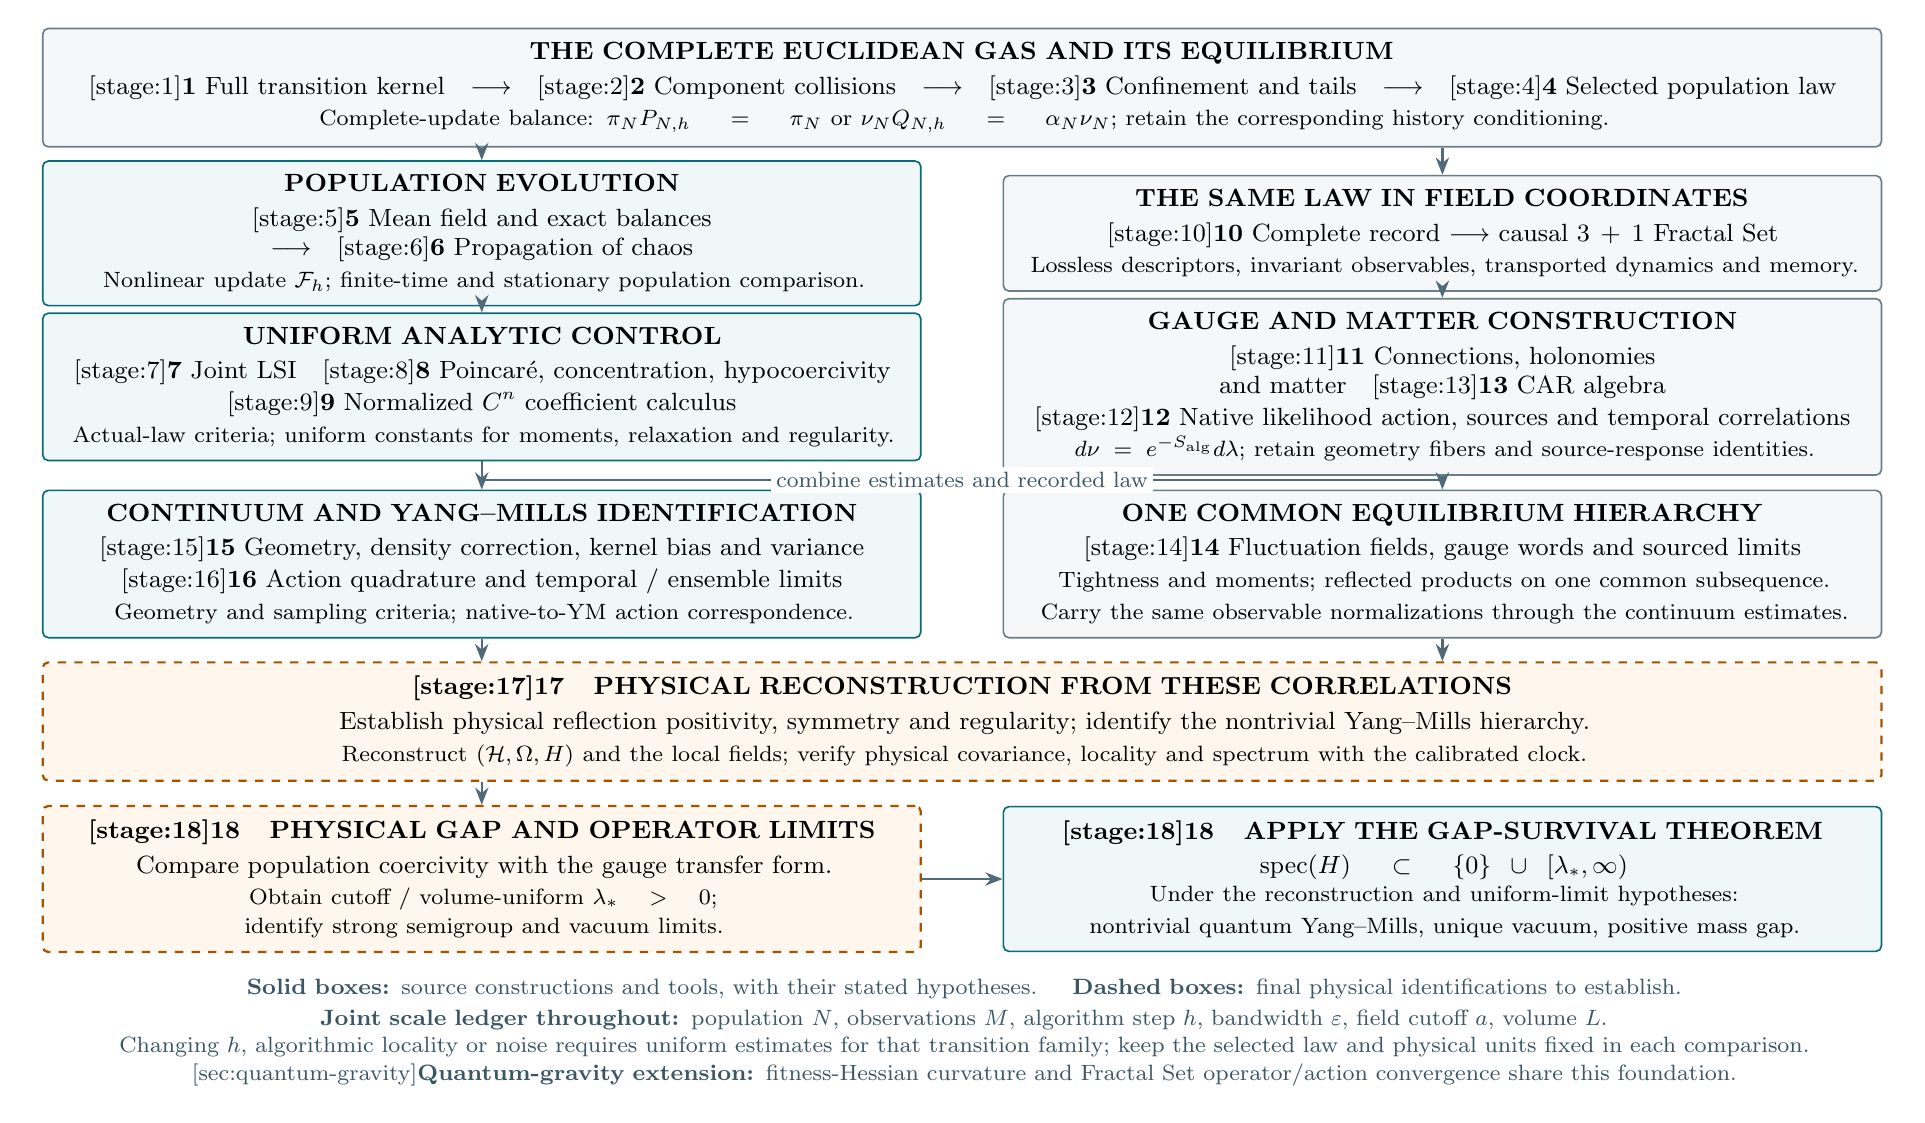
\begin{tikzpicture}[
  x=1cm,y=1cm,
  every node/.style={font=\fontsize{9}{10.5}\selectfont,align=center},
  box/.style={draw=ink!65,fill=ink!4,rounded corners=2pt,line width=.6pt,
    text width=10.8cm,minimum height=1.22cm,inner sep=5pt},
  full/.style={box,text width=23cm},
  control/.style={box,draw=teal!85!black,fill=teal!6},
  target/.style={box,draw=orange!65!black,fill=orange!7,dashed,line width=.8pt},
  flow/.style={-{Stealth[length=2.2mm,width=1.7mm]},draw=ink!75,line width=.8pt},
  link/.style={draw=ink!75,line width=.8pt},
  note/.style={font=\fontsize{8}{9}\selectfont,text=ink!85},
]
\node[full] (gas) at (0,0) {
  \textbf{THE COMPLETE EUCLIDEAN GAS AND ITS EQUILIBRIUM}\\[2pt]
  \hyperref[stage:1]{\textbf{1} Full transition kernel}\quad$\longrightarrow$\quad
  \hyperref[stage:2]{\textbf{2} Component collisions}\quad$\longrightarrow$\quad
  \hyperref[stage:3]{\textbf{3} Confinement and tails}\quad$\longrightarrow$\quad
  \hyperref[stage:4]{\textbf{4} Selected population law}\\[1pt]
  {\fontsize{8}{9}\selectfont Complete-update balance: $\pi_NP_{N,h}=\pi_N$ or $\nu_NQ_{N,h}=\alpha_N\nu_N$; retain the corresponding history conditioning.}
};

\node[control] (meanfield) at (-6.1,-1.85) {
  \textbf{POPULATION EVOLUTION}\\[2pt]
  \hyperref[stage:5]{\textbf{5} Mean field and exact balances}\quad$\longrightarrow$\quad
  \hyperref[stage:6]{\textbf{6} Propagation of chaos}\\[1pt]
  {\fontsize{8}{9}\selectfont Nonlinear update $\mathcal F_h$; finite-time and stationary population comparison.}
};
\node[box] (record) at (6.1,-1.85) {
  \textbf{THE SAME LAW IN FIELD COORDINATES}\\[2pt]
  \hyperref[stage:10]{\textbf{10} Complete record $\longrightarrow$ causal $3+1$ Fractal Set}\\[1pt]
  {\fontsize{8}{9}\selectfont Lossless descriptors, invariant observables, transported dynamics and memory.}
};

\node[control,minimum height=1.42cm] (tools) at (-6.1,-3.8) {
  \textbf{UNIFORM ANALYTIC CONTROL}\\[2pt]
  \hyperref[stage:7]{\textbf{7} Joint LSI}\quad
  \hyperref[stage:8]{\textbf{8} Poincar\'e, concentration, hypocoercivity}\\[1pt]
  \hyperref[stage:9]{\textbf{9} Normalized $C^n$ coefficient calculus}\\[1pt]
  {\fontsize{8}{9}\selectfont Actual-law criteria; uniform constants for moments, relaxation and regularity.}
};
\node[box,minimum height=1.42cm] (fields) at (6.1,-3.8) {
  \textbf{GAUGE AND MATTER CONSTRUCTION}\\[2pt]
  \hyperref[stage:11]{\textbf{11} Connections, holonomies and matter}\quad
  \hyperref[stage:13]{\textbf{13} CAR algebra}\\[1pt]
  \hyperref[stage:12]{\textbf{12} Native likelihood action, sources and temporal correlations}\\[1pt]
  {\fontsize{8}{9}\selectfont $d\nu=e^{-S_{\rm alg}}d\lambda$; retain geometry fibers and source-response identities.}
};

\coordinate (join) at (0,-4.98);
\node[control,minimum height=1.35cm] (continuum) at (-6.1,-6.05) {
  \textbf{CONTINUUM AND YANG--MILLS IDENTIFICATION}\\[2pt]
  \hyperref[stage:15]{\textbf{15} Geometry, density correction, kernel bias and variance}\\[1pt]
  \hyperref[stage:16]{\textbf{16} Action quadrature and temporal / ensemble limits}\\[1pt]
  {\fontsize{8}{9}\selectfont Geometry and sampling criteria; native-to-YM action correspondence.}
};
\node[box,minimum height=1.35cm] (hierarchy) at (6.1,-6.05) {
  \textbf{ONE COMMON EQUILIBRIUM HIERARCHY}\\[2pt]
  \hyperref[stage:14]{\textbf{14} Fluctuation fields, gauge words and sourced limits}\\[1pt]
  {\fontsize{8}{9}\selectfont Tightness and moments; reflected products on one common subsequence.}\\[1pt]
  {\fontsize{8}{9}\selectfont Carry the same observable normalizations through the continuum estimates.}
};

\node[target,text width=23cm,minimum height=1.3cm] (reconstruction) at (0,-8.05) {
  \textbf{\hyperref[stage:17]{17\quad PHYSICAL RECONSTRUCTION FROM THESE CORRELATIONS}}\\[2pt]
  Establish physical reflection positivity, symmetry and regularity; identify the nontrivial Yang--Mills hierarchy.\\[1pt]
  {\fontsize{8}{9}\selectfont Reconstruct $(\mathcal H,\Omega,H)$ and the local fields; verify physical covariance, locality and spectrum with the calibrated clock.}
};
\node[target,minimum height=1.35cm] (gapinput) at (-6.1,-10.05) {
  \textbf{\hyperref[stage:18]{18\quad PHYSICAL GAP AND OPERATOR LIMITS}}\\[2pt]
  Compare population coercivity with the gauge transfer form.\\[1pt]
  {\fontsize{8}{9}\selectfont Obtain cutoff / volume-uniform $\lambda_*>0$; identify strong semigroup and vacuum limits.}
};
\node[control,minimum height=1.35cm] (conclusion) at (6.1,-10.05) {
  \textbf{\hyperref[stage:18]{18\quad APPLY THE GAP-SURVIVAL THEOREM}}\\[2pt]
  $\Spec(H)\subset\{0\}\cup[\lambda_*,\infty)$\\[1pt]
  {\fontsize{8}{9}\selectfont Under the reconstruction and uniform-limit hypotheses:\\[1pt]nontrivial quantum Yang--Mills, unique vacuum, positive mass gap.}
};

\draw[flow] (gas.south -| meanfield.north) -- (meanfield.north);
\draw[flow] (gas.south -| record.north) -- (record.north);
\draw[flow] (meanfield.south) -- (tools.north);
\draw[flow] (record.south) -- (fields.north);
\draw[link] (tools.south) -- (-6.1,-4.98) -- (join);
\draw[link] (fields.south) -- (6.1,-4.98) -- (join);
\fill[ink!75] (join) circle (1.2pt);
\draw[flow] (-6.1,-4.98) -- (continuum.north);
\draw[flow] (6.1,-4.98) -- (hierarchy.north);
\node[note,fill=white,inner sep=2pt] at (0,-4.98) {combine estimates and recorded law};
\draw[flow] (continuum.south) -- (reconstruction.north -| continuum.south);
\draw[flow] (hierarchy.south) -- (reconstruction.north -| hierarchy.south);
\draw[flow] (reconstruction.south -| gapinput.north) -- (gapinput.north);
\draw[flow] (gapinput.east) -- (conclusion.west);

\node[note,text width=23.5cm] at (0,-12.0) {
  \textbf{Solid boxes:} source constructions and tools, with their stated hypotheses.
  \quad\textbf{Dashed boxes:} final physical identifications to establish.\\[2pt]
  \textbf{Joint scale ledger throughout:} population $N$, observations $M$, algorithm step $h$,
  bandwidth $\varepsilon$, field cutoff $a$, volume $L$.\\[1pt]
  Changing $h$, algorithmic locality or noise requires uniform estimates for that transition family; keep the selected law and physical units fixed in each comparison.\\[1pt]
  \hyperref[sec:quantum-gravity]{\textbf{Quantum-gravity extension:} fitness-Hessian curvature and Fractal Set operator/action convergence share this foundation.}
};
\end{tikzpicture}
\end{center}
\end{landscape}
\clearpage

\section*{Equilibrium thermodynamics and the field state}
\phantomsection\label{sec:equilibrium-thermodynamics}
\addcontentsline{toc}{section}{Equilibrium thermodynamics and the field state}
The equilibrium construction fixes both the population statistics and the temporal law from which the field theory is derived. Its successive objects are the thermal reference, the selected law of the complete population update, the stationary mean field and its fluctuations, and the induced gauge and matter history. The following chain connects these objects to the physical reconstruction in Stages~\ref{stage:17}--\ref{stage:18}.

\subsection*{Thermal balance and the complete population law}
For the conservative kinetic Langevin model, the gradient force, velocity friction and matching Gaussian noise give
\[
\theta=\frac{\sigma_v^2}{2\gamma},\qquad
m_U(dx\,dv)=Z_U^{-1}
\exp\!\left[-\frac{U(x)+|v|^2/2}{\theta}\right]dx\,dv.
\]
Confinement makes the partition function finite. Hamiltonian transport preserves the kinetic energy plus potential, while friction and noise balance at temperature \(\theta\). This is the explicit kinetic Gibbs reference \hyperref[src:def-gibbs-kinetic]{[R1]}. The kinetic LSI theorem incorporates its Gaussian velocity factor and gives \(C_0=\max\{C_x,\theta\}\) \hyperref[src:thm-kinetic-lsi]{[R2]}.

The complete configured update determines the population equilibrium through
\[
\pi_NP_{N,h}=\pi_N,
\qquad
\nu_NQ_{N,h}=\alpha_N\nu_N,
\quad 0<\alpha_N\le1.
\]
The first identity selects the conservative invariant law; the second selects the killed process's quasi-stationary law. A Gibbs profile for either law is identified by inserting that profile into its complete equation, with cloning, collision, cap and boundary stages retained. The source supplies a quantitative version: for a proposed probability \(g\), a killed block \(Q\), \(b=gQ1>0\), and a normalized block map contracting total variation by \(r<1\),
\[
\|g-\nu_N\|_{\rm TV}
\le\frac{\|gQ-bg\|_{\rm TV}}{b(1-r)}.
\]
Thus exact balance identifies the Gibbs law, and the evaluated balance residual controls an approximate Gibbs identification \hyperref[src:thm-qsd-gibbs]{[R3]}. These equations connect the thermal reference to the selected population ensemble of Stage~\ref{stage:4}.

\subsection*{Population thermodynamics supplies uniform coercivity}
For an identified joint Gibbs law \(d\pi_N=Z_N^{-1}e^{-V_N}dz\), uniform curvature \(\nabla^2V_N\succeq\rho_*I\) gives \(C_*=1/\rho_*\). A concrete strongly convex specialization in the book is
\begin{align*}
V_N(z)&=\sum_iV_0(z_i)
 +\frac{\epsilon_{\rm int}}{N}\sum_{i<j}W(z_i,z_j),\\
\rho_*&=\rho_0-\epsilon_{\rm int}L_W>0,
\end{align*}
where \(\nabla^2V_0\succeq\rho_0I\) and the pair Hessian has norm at most \(L_W\). The normalized interaction preserves this curvature independently of \(N\) \hyperref[src:prop-kl-joint-interaction-curvature]{[R4]}. Product, bounded joint tilt and contractive-flow criteria provide the other population-uniform routes \hyperref[src:cor-n-uniform-lsi]{[R5]}.

For the continuous coordinates of that same law, these estimates imply
\begin{align*}
\Ent_{\pi_N}(f^2)&\le2C_*\int|\nabla f|^2\,d\pi_N,\\
\Var_{\pi_N}(F)&\le C_*\int|\nabla F|^2\,d\pi_N,\\
\Var_{\pi_N}(L_N\varphi)&\le
 \frac{C_*\operatorname{Lip}(\varphi)^2}{N}.
\end{align*}
The full gradient retains every position and velocity coordinate; discrete alive/dead marks carry the additional status entropy of Stage~\ref{stage:7}. The empirical variance estimate controls an interacting population directly \hyperref[src:cor-quantitative-lsi-final]{[R6]}.

The evolution uses this coercivity through the modified kinetic entropy. The common-target theorem gives a proved route when the cloning kernel preserves the kinetic equilibrium and its Fisher amplification satisfies the stated bound \hyperref[src:thm-main-kl-convergence]{[R7]}. The full-law theorem instead combines the actual stationary law, complete cloning and killing source, and a negative modified-entropy derivative; its conclusion is
\[
D_{\rm KL}(\mu_t\Vert\nu_N)
\le\Phi_{G_N}(h_0)e^{-r_Nt},
\qquad
r_N=\frac{\delta_N}{C_N/2+g_{+,N}}.
\]
Uniform bounds on \(C_N\), \(g_{+,N}\) and \(\delta_N^{-1}\) retain a positive population-independent relaxation rate \hyperref[src:thm-kl-convergence-euclidean]{[R8]}. The selected discrete update uses the full-step entropy estimates described in Stage~\ref{stage:8}.

\subsection*{The stationary mean field and its controlled fluctuations}
The nonlinear map \(\mathcal F_h\) is computed from the same complete update. Under the stationary-chaos hypotheses of Stage~\ref{stage:6}, the selected population law has a deterministic macroscopic limit,
\[
\mu_*=\mathcal F_h(\mu_*),\qquad
L_N\varphi\longrightarrow\mu_*\varphi
\quad\text{in probability and every finite }L^p
\]
for bounded continuous \(\varphi\) \hyperref[src:thm-thermodynamic-limit]{[R9]}. The marginal LSI passes to the limiting law on its stated test-function domain \hyperref[src:cor-kl-lsi-mean-field-limit]{[R10]}. Smooth normalized mean-field integrals then supply the metric, force and reconstruction coefficients in Stage~\ref{stage:9}.

Retaining the centered fluctuations gives
\[
\Xi_N(\varphi)=\sqrt N
\bigl(L_N\varphi-\mathbb E_{\pi_N}L_N\varphi\bigr),
\qquad
\mathbb E|\Xi_N(\varphi)|^2
\le C_*\operatorname{Lip}(\varphi)^2.
\]
Their drift and covariance are calculated from the actual kernel, including the shared collision rotation and cloning writes. The mean field controls the background coefficients; the fluctuation hierarchy retains the random field. Moment bounds, normalized derivative estimates and the two continuum estimator bounds of Stage~\ref{stage:15} control the passage to the continuum on the selected observation law.

\subsection*{The equilibrium history induces the field state and action}
Start the conservative record at \(\pi_N\), or use the specified QSD window or Doob history. The complete transition determines every temporal correlation. For an invariant law and centered channel observables \(\widetilde f_a\), the recorded-time correlator is
\[
C_{ab}(\ell)=
\langle\widetilde f_a,P_{N,h}^{\ell}\widetilde f_b\rangle_{L^2(\pi_N)},
\qquad t_\ell=\ell\Delta t.
\]
This is the equilibrium correlator identity used in Stage~\ref{stage:17} \hyperref[src:thm-effective-twistor-spectral-meaning]{[R11]}. The spatial coordinates remain in \(\mathbb R^3\), and the temporal separation is measured by the recorded algorithmic clock.

Push the complete history law \(P^{\rm hist}\) and its specified reference \(R^{\rm hist}\) through the Fractal Set descriptor \(Y=\mathscr D(\omega)\). With \(\lambda=\mathscr D_*R^{\rm hist}\), the action theorem gives
\begin{gather*}
e^{-S_{\rm alg}(y)}=
\mathbb E_{R^{\rm hist}}\!\left[
\frac{dP^{\rm hist}}{dR^{\rm hist}}\middle|Y=y\right],
\qquad d\nu=e^{-S_{\rm alg}}d\lambda,\\
\varpi(O)=\mathbb E_{P^{\rm hist}}O(Y)=\int O\,d\nu.
\end{gather*}
The induced state \(\varpi\), action, source derivatives and temporal correlations all come from this record likelihood \hyperref[src:thm-ym-recorded-action-emergence]{[R12]}. Geometry-fiber disintegration retains the normalization needed to recover the same joint law \hyperref[src:thm-ym-native-geometry-fiber-action]{[R13]}. Stage~\ref{stage:12} computes its predictive evolution and source response, and Stage~\ref{stage:16} carries the sourced action and correlations through the controlled limits.

Thermodynamic response is also explicit. For bounded observables \(A,B\) and the specified equilibrium tilt \(d\pi_s=Z(s)^{-1}e^{\beta sB}d\pi\), the susceptibility formula is \hyperref[src:prop-fluctuation-dissipation]{[R14]}
\[
\left.\frac{d}{ds}\pi_s(A)\right|_{s=0}
=\beta\operatorname{Cov}_{\pi}(A,B)
\]
A perturbation of the actual transition has the stationary Poisson-response formula already given in Stage~\ref{stage:12} \hyperref[src:thm-algorithmic-stationary-response]{[R15]}. Each response therefore specifies both the perturbed law and the evolution used to compute it.

\subsection*{Physical reconstruction and survival of the gap}
Stages~\ref{stage:17}--\ref{stage:18} use the limiting equilibrium hierarchy just constructed. The temporal reflection is \(\Theta:(t,x)\mapsto(-t,x)\) in its recorded clock. Identify its positive reflection pairing and transfer representation on the retained gauge and matter observables; the reconstruction then supplies the physical Hilbert space, vacuum and self-adjoint Hamiltonian. For a centered self-adjoint channel in the positive-transfer representation with a unique vacuum and complete orthonormal energy basis, the source gives \hyperref[src:cor-effective-twistor-positive-transfer]{[R16]}
\[
C_{aa}(\ell)=\sum_{E_j>0}
|\langle j|\widehat f_a|0\rangle|^2
e^{-E_j\ell\Delta t}
\]
Verify the accompanying spacetime covariance and field-axiom hypotheses on this same limiting hierarchy.

To turn population coercivity into the physical mass gap, identify the physical Hamiltonian form and its norm so that the transported estimates give
\begin{gather*}
\mathcal E_a(\psi,\psi)=\|H_a^{1/2}\psi\|^2
\ge\lambda_*\|\psi\|^2,
\qquad\lambda_*>0,\\
\psi\in\operatorname{Dom}(H_a^{1/2})\cap\Omega_a^\perp,
\end{gather*}
uniformly along the chosen cutoff and volume family. This is the specified form comparison between the thermodynamic control and the physical transfer Hamiltonian. The source's gap-survival theorem \hyperref[src:thm-mass-gap-rg-fixed-point]{[R17]} then passes the estimate through the strong semigroup and vacuum limits of Stage~\ref{stage:18}, giving
\[
\Spec(H)\subset\{0\}\cup[\lambda_*,\infty),
\qquad \ker H=\mathbb C\Omega
\]
The selected population law defines the field state, its evolution and its quantitative continuum controls. The final representation and form identifications place those controls on the physical Yang--Mills theory.


\section{Fix the Euclidean gas}
\label{stage:1}
Begin with the complete marked swarm \(S=((x_i,v_i,a_i))_{i=1}^N\) with positions, velocities, and alive/dead status. Dead slots retain their coordinates. Freeze the input frame for measurement, fitness, donor choice, and acceptance; this fixes the update order and prevents updated donor coordinates from leaking into the same cloning stage.

The canonical update samples one measurement companion, computes regularized population statistics and positive logistic fitness, samples a cloning donor, and accepts according to the frozen score. Accepted edges define connected collision components. Copy recipient positions with Gaussian jitter, rotate each component about its center-of-mass velocity, apply BAOAB and final position noise, cap velocities, and classify the terminal boundary once.

Declare the absorbing or conservative configuration, the objective and force, the noise laws, the internal marks, and all parameter floors. If historical donors or mutable providers are used, include their memory in the complete state. This stage fixes the stochastic object used throughout the program.


\begin{gather*}
E=\mathbb R^d\times\overline B_V\times\{0,1\},\qquad S\in E^N,\qquad L_N=\frac1N\sum_{i=1}^N\delta_{z_i},\quad z_i=(x_i,v_i,a_i).
\end{gather*}
\subsection*{Proof mechanism}
Construct the companion and donor kernels by normalizing strictly positive weights against the alive population. The regularized standard deviations keep the score maps defined on constant populations. Condition on the frozen marks and accepted-edge graph, then compose the collision, Gaussian, deterministic kinetic, cap, and classification kernels. Integrating these conditional kernels gives \(P_{N,h}\). Its path law is the initial law times the ordered product of the complete transition kernels. Record coverage is fixed at this point, so later likelihood calculations integrate the randomness that actually produced the path.
\subsection*{Analytic inputs}
Marked Markov state; positive fitness and normalization floors; bounded comparison features; Gaussian innovations; Feller regularity. The Euclidean Gas Update is the defining algorithm in convergence\_program/02\_euclidean\_gas.md, label alg-euclidean-gas.
\paragraph{Stage output.} A complete finite-particle transition and a record contract that specifies every random choice and intermediate stage. Subsequent mean-field and field constructions use this kernel.

\section{Resolve cloning and collision geometry}
\label{stage:2}
An accepted donor edge changes the recipient position and joins its endpoints into a collision component. Overlapping groups form a single connected component. The shared orthogonal rotation acts on the component relative velocities, so each walker has one velocity destination.

The tagged-walker population description must retain its random collision neighborhood. Strict fitness increase along accepted live edges supplies component control in the canonical current-frame construction. Rooted component convergence connects these finite neighborhoods to the limiting collision law.

Compute momentum, restitution energy, and the cross-walker covariance created by the shared rotation. Retain these terms in fluctuation and mean-field calculations: the noises of members of one component are correlated.


\begin{gather*}
\widetilde v_i=\overline v_C+\alpha R_C(v_i-\overline v_C),\qquad R_C\sim\mathrm{Haar}(O(d)),
\quad \sum_{i\in C}\widetilde v_i=\sum_{i\in C}v_i.
\end{gather*}
\subsection*{Proof mechanism}
For a component \(C\), the centered velocities satisfy \(\sum_{i\in C}(v_i-\overline v_C)=0\). Orthogonality preserves their squared norm and Haar symmetry gives zero mean for the rotated component. Taking traces in the rotationally invariant covariance identity gives
\[\operatorname{Cov}(\widetilde v_i,\widetilde v_j\mid C)
=\frac{\alpha^2}{d}\bigl[(v_i-\overline v_C)\cdot(v_j-\overline v_C)\bigr]I_d.\]
For the population limit, truncate the rooted accepted-edge component, compare its finite exploration law with the limiting rooted law, and remove the truncation using the proved component moments. The two-root calculation controls the empirical variance. These steps identify the collision term without replacing component rotations by independent row noise.
\subsection*{Analytic inputs}
Accepted-edge graph; rooted-component truncation; moment bounds at every component order; shared Haar rotation; self-exclusion correction; two-root independence in the population limit.
\subsection*{Source results}
\begin{itemize}
\item \textbf{Component momentum, energy, and shared covariance}~\hyperref[src:thm-mean-field-component-identities]{[R18]}. Component momentum, energy, and shared covariance.
\item \textbf{One-step collision consistency}~\hyperref[src:thm-mean-field-one-step-consistency]{[R19]}. One-step collision consistency for the rooted population law.
\end{itemize}
\paragraph{Stage output.} The actual collision law and its conservation, moment, and covariance data. These feed the fixed-step population map and its fluctuation equations.

\section{Control confinement, moments, and tails}
\label{stage:3}
Combine cloning displacement with kinetic transport to derive a Foster-Lyapunov estimate for the complete update. Choose positive weights for the component drift inequalities and evaluate the resulting rate and source. Iterate the drift to obtain finite-time and stationary moment budgets.

The structural landscape chapter also derives selection-driven confinement from accepted inward and outward donor fluxes. Its complete moment inequality retains the selection excess and the kinetic force-growth coefficients. It provides an explicit criterion for contracting moments without a prescribed restoring trap.

Use these moment bounds to localize unbounded reward estimates, control population coverage failures, obtain tightness, and justify uniform integrability. The entropy-to-tail and population-fraction bounds give a second quantitative route to controlling the mass of poorly covered or distant regions.


\begin{gather*}
P_NW_p\le r_pW_p+B_p+a_pE_p,\qquad r_p<1,\\
\mathbb EW_p(S_n)\le r_p^n\mathbb EW_p(S_0)+\frac{B_p+a_p\overline e_p}{1-r_p}(1-r_p^n).
\end{gather*}
\subsection*{Proof mechanism}
Evaluate the copying increment \(|x_j|^p-|x_i|^p\) under accepted donor flux. Lower bounds on inward core flux and upper bounds on outward tail flux give a signed selection drift. Add cloning jitter through Gaussian radial moments, then propagate through the actual kinetic position update using the force-growth and cap bounds. The remainder \(E_p\) records coverage or class failures. Iterating the resulting affine recurrence gives the displayed moment budget. Markov's inequality turns higher moments into quantitative tail localization; the entropy-floor calculation gives additional tail and population-fraction estimates for the normalized joint positional law.
\subsection*{Analytic inputs}
Foster-Lyapunov drift; positive-weight spectral criterion; Gaussian radial moments; regional selection flux; coverage and tail budgets; entropy confinement floor.
\subsection*{Source results}
\begin{itemize}
\item \textbf{Foster-Lyapunov drift for the composed kernel}~\hyperref[src:thm-foster-lyapunov-main]{[R20]}. Composes the drift estimates at the level of the actual kernel.
\item \textbf{Fully evaluated selection-driven moment drift without a prescribed restoring trap}~\hyperref[src:thm-slceg-full-moment]{[R21]}. Evaluates selection-driven moment drift, including the zero-restoring-trap regime.
\item \textbf{Entropy contraction to an explicit confinement floor}~\hyperref[src:thm-slce-entropy-floor]{[R22]}. Converts verified selection into entropy contraction toward an explicit confinement floor.
\end{itemize}
\subsection*{Structural transport and mass--shape control}
The positional transport chapter derives the centered structural control from the cloning variance reset and carries the barycenter separately in its full \(W_2\) decomposition. The structural landscape chapter evaluates the signed Keystone, collision, and kinetic terms for the complete update. These results retain the inward selection flux, the donor-normalization costs, and the actual force increments in the same one-step ledger.

The mass, Hellinger, and transport chapter combines the alive mass with normalized shape. For finite measures \(m\rho\) and \(m_*\rho_*\), it proves the exact mass--shape identity
\[
H^2(m\rho,m_*\rho_*)
=(\sqrt m-\sqrt{m_*})^2+\sqrt{mm_*}\,H^2(\rho,\rho_*).
\]
It combines this with entropy-to-Hellinger and entropy-to-transport inequalities and also bounds the canonical Hellinger--Kantorovich distance. Safe-walker survival, concentration of alive mass, and convergence of the conditioned shape therefore control separate parts of the finite-measure error. This is the population normalization used in the convergence analysis.
\subsection*{Results supplying these constructions}
\begin{itemize}
\item \textbf{Structural/Barycenter Split for Full \(W_2\)}~\hyperref[src:thm-full-w2-split]{[R23]}. Carries the barycenter and centered structural terms in full transport control.
\item \textbf{Joint convergence of mass and shape}~\hyperref[src:thm-hk-convergence-main-assembly]{[R24]}. Assembles convergence of alive mass and normalized shape.
\item \textbf{Finite-horizon survival from safe-walker estimates}~\hyperref[src:thm-exponential-survival]{[R25]}. Controls finite-horizon survival through the safe-walker estimates.
\end{itemize}
\paragraph{Stage output.} Population-uniform physical moment and tail controls for the chosen parameter regime. These support tightness, stationary limits, smooth reconstruction, and control of field moments.

\section{Select the stationary or conditioned ensemble}
\label{stage:4}
For the conservative process, the drift and common-mass estimates give convergence to its identified invariant law. For the killed process, the surviving-block results give the selected QSD and its survival eigenvalue. The finite-window and Doob constructions specify which conditioned history is observed.

The recorded observation time is \(t_n=n\Delta t\), where \(\Delta t\) includes any configured recording stride and fixed physical-unit calibration. Burn-in advances this same dynamics to the selected equilibrium ensemble. Subsequent windows retain their algorithmic time differences and all recorded transition data.

The Yang--Mills chapter computes the selected QSD window weights and its relaxation error. The equilibrium law supplies the starting ensemble; the complete transition supplies every temporal correlation used below.

\begin{gather*}
\pi_NP_{N,h}=\pi_N,\qquad \nu_NQ_{N,h}=\alpha_N\nu_N,\quad 0<\alpha_N\le1.
\end{gather*}
\subsection*{Proof mechanism}
Iterate the weighted drift to enter the controlled region, then apply the appropriate common-mass or surviving-block comparison. In the conservative case, the coupling contracts a weighted distance and yields an invariant probability. In the killed case, normalized block iteration yields the selected eigenmeasure. For a QSD window, multiply the killed transitions and divide by the window survival probability. Successive survival factors cancel in the selected-history identity. Comparing an actual relaxed window with this eigenmeasure window introduces the explicit survival amplification, bounded in the chapter by \(2\alpha_N^{-w}\delta_n\) for a \(w\)-step window.
\subsection*{Analytic inputs}
Weighted Harris coupling; surviving-block minorization; eigenmeasure identities; survival normalization; total-variation window comparison.
\subsection*{Source results}
\begin{itemize}
\item \textbf{A weighted coupling form of Harris' argument}~\hyperref[src:thm-convergence-conservative-harris]{[R26]}. Conservative mixing from the declared drift and coupling inputs.
\item \textbf{QSD convergence from a two-sided surviving-block bound}~\hyperref[src:thm-main-convergence]{[R27]}. QSD convergence from a two-sided surviving-block bound.
\item \textbf{Relaxation to the selected law of a recorded gauge window}~\hyperref[src:thm-ym-qsd-window-relaxation]{[R28]}. Transfers the gas relaxation rate to a selected recorded gauge window.
\end{itemize}
\paragraph{Stage output.} A selected long-time law and its exact history-window law, together with burn-in and conditioning errors. Field reconstruction takes expectations under this specified ensemble.

\section{Derive the population law and exact field equations}
\label{stage:5}
Pass from the swarm empirical measure to a nonlinear population law on marked one-slot states. Keep the alive restriction and its normalized donor law distinct from the full population law, because dead positions and velocities affect revival and collision behavior.

The construction first samples the measurement mark, then applies population standardization and fitness, then samples accepted edges and the limiting collision neighborhood. It finally composes the actual kinetic stages and terminal classification. Averaging the measurement before its nonlinear acceptance step would change the map.

The resulting population equation is discrete at the fixed configured timestep. Derive its mass balance, weak field balances, positive alive mass, and finite-horizon moments. Stationary solutions are fixed points of this map. A continuous-time generator requires its own local consistency calculation if h is later changed.


\begin{gather*}
\mu_{n+1}=\mathcal F_h(\mu_n),\qquad m(\mu)=\mu(a=1),\qquad \rho_\mu=\frac{\mu^a}{m(\mu)}.
\end{gather*}
\subsection*{Proof mechanism}
Disintegrate a representative row into its measurement mark, frozen fitness, donor gate, rooted collision component, and independent kinetic innovations. Integrate the root output against this product of conditional laws to define \(\mathcal F_h\). Positivity and total mass follow from kernel composition. Gaussian final position noise makes terminal box classification continuous after averaging and supplies positive alive mass. Polynomial growth of reward is handled by the propagated moments. The weak mass and field balances follow by testing the same root input-output coupling; each term belongs to a declared stage of the complete update.
\subsection*{Analytic inputs}
Normalized companion integrals; measurement marks; finite limiting collision neighborhoods; exact composition of BAOAB, diffusion, cap, and classification.
\subsection*{Source results}
\begin{itemize}
\item \textbf{The fixed-step mean-field equation}~\hyperref[src:thm-mean-field-equation]{[R29]}. The exact fixed-step mean-field equation.
\item \textbf{Exact mass and weak field balances}~\hyperref[src:thm-mass-conservation]{[R30]}. Exact mass and weak field balances for the full population update.
\end{itemize}
\subsection*{The finite algorithm already has field equations}
The field-equations chapter derives the hierarchy directly from the configured donor, cloning, innovation, and boundary maps. Its full marked state retains current and historical donor data, eligibility, provider state, and the inputs needed by the next update. On this state, its marked field and age transport are exact.

For any square-integrable vector observable \(A\), the complete kernel gives
\begin{align*}
b_A(S)&=P_{N,h}A(S)-A(S),\\
\Gamma_A(S)&=P_{N,h}(AA^\top)(S)-P_{N,h}A(S)P_{N,h}A(S)^\top,\\
A(S_{n+1})-A(S_n)&=b_A(S_n)+\eta_{n+1},
\end{align*}
with \(\mathbb E[\eta_{n+1}\mid S_n]=0\) and conditional covariance \(\Gamma_A(S_n)\). The same formula applies to metric probes and gauge readouts. Fourier tests and the marked characteristic functional give the exact moment and field-correlation hierarchy, retaining the configured innovation law and cross-walker dependence.

For a row transition \((x,v,a)\mapsto(y,w,b)\), deposit along the segment from \(x\) to \(y\). The fundamental theorem of calculus gives the distributional density and current balances. Summing over the actual stages telescopes to
\[
\rho_{n+1}-\rho_n+\operatorname{div}\mathcal J_\rho=\mathcal S_\rho,
\qquad
j_{n+1}-j_n+\operatorname{div}\mathcal J_j=\mathcal S_j.
\]
All source and transport terms are computed from the executed update. The coupled-field theorem combines these mechanical equations with the population, history, Hessian metric, and thermostat covariance. Configured algorithm variants retain their own stage ordering and coefficients in these identities.
\subsection*{Results supplying these constructions}
\begin{itemize}
\item \textbf{Explicit finite-step population law}~\hyperref[src:thm-algorithmic-explicit-transition]{[R31]}. Explicit finite-step population law for the configured complete state.
\item \textbf{Exact field characteristics and moment hierarchy}~\hyperref[src:thm-algorithmic-field-characteristics]{[R32]}. Exact characteristics, characteristic functional, and moment hierarchy.
\item \textbf{Finite-step observable equation and fluctuation covariance}~\hyperref[src:thm-algorithmic-observable-increment]{[R33]}. Exact drift and conditional fluctuation covariance of derived observables.
\item \textbf{Exact discrete spatial density and momentum equations}~\hyperref[src:thm-algorithmic-spatial-field-equations]{[R34]}. Exact finite-step spatial density and momentum balances.
\item \textbf{Coupled population, mechanical, and metric fields}~\hyperref[src:thm-algorithmic-coupled-field-system]{[R35]}. The coupled population, mechanical, and metric field system.
\end{itemize}
\paragraph{Stage output.} The nonlinear population update, its sampled interaction law, and its exact balance relations. This is the background law for the smooth field and fluctuation constructions.

\section{Control particles, observation time, and stationarity}
\label{stage:6}
Prove one-step consistency of the finite update with the nonlinear population map, including measurement concentration, collision-component convergence, and boundary/revival contributions. Iterate to obtain finite-horizon propagation of chaos.

For long times, use the structural landscape results appropriate to the declared regime. The weighted active-contraction branch provides a unique stationary population law and a population-independent attraction rate. Its trajectory corollary supplies uniform-time approximation, stationary chaos, and commuting population/time limits with explicit initial moment control.

The growing-horizon branch instead supplies trajectory approximation through a diverging observation horizon using higher moments and the actual consistency constants. This provides a controlled joint population/time limit without assuming attraction. Keep the branch used by the field ensemble explicit.


\begin{gather*}
\left|\mathbb E[L'_N\varphi\mid S]-\mathcal F_h(L_N(S))\varphi\right|
\le\frac{2\|\varphi\|_\infty B_*}{\sqrt N},\\
\mathbb E\!\left[|L'_N\varphi-\mathcal F_h(L_N(S))\varphi|^2\mid S\right]
\le\frac{A_\varphi+4\|\varphi\|_\infty^2B_*^2}{N}.
\end{gather*}
\subsection*{Proof mechanism}
Condition on the input array and estimate the realized measurement-normalization fluctuations. Couple the resulting donor and gate laws, use rooted-component estimates for the collision response, and apply conditional concentration to independent kinetic innovations. This proves the displayed one-step bias and mean-square bounds at the actual empirical input. Continuity of \(\mathcal F_h\) and a countable determining class give finite-horizon iteration. For stationary limits, combine one-step consistency with population attraction and tightness. In the weighted-contraction branch, expand two iterates and verify the source condition
\[q_w=1-\epsilon_2/2+2B_wL_{\rm rem}+L_{\rm rem}^2<1.\]
The growing-horizon branch instead propagates its explicit error recursion and high-moment budget to a diverging observation horizon.
\subsection*{Analytic inputs}
Rooted collision convergence; one-step bias and mean-square consistency; conditional concentration; weighted TV contraction; finite-row chaos; growing-horizon error recursion.
\subsection*{Source results}
\begin{itemize}
\item \textbf{Finite-horizon propagation of chaos for the actual update}~\hyperref[src:thm-chaos-finite-time-consistency]{[R36]}. Finite-horizon propagation of chaos for the actual update.
\item \textbf{Closed full-law convergence with unbounded raw reward}~\hyperref[src:thm-slcw-active-contraction]{[R37]}. Closed full-law population convergence with unbounded raw reward.
\item \textbf{Uniform-time trajectories, stationary chaos and commuting limits}~\hyperref[src:cor-slcw-trajectories]{[R38]}. Uniform-time trajectories, stationary chaos, and commuting limits.
\item \textbf{Uniform trajectory approximation through a diverging horizon}~\hyperref[src:thm-slcgt-growing-trajectory]{[R39]}. A separate explicit trajectory estimate through a diverging horizon.
\end{itemize}
\subsection*{Exchangeability connects the empirical law to tagged fields}
Kernel permutation symmetry and uniqueness give exchangeability of the selected finite law. The exchangeability chapter derives the finite empirical-mixture representation and proves that a deterministic empirical limit gives fixed-row chaos. It also evaluates the finite-population covariance exactly:
\[
\operatorname{Cov}(g(Z_1),h(Z_2))
=\frac{N\operatorname{Cov}(L_Ng,L_Nh)
-\operatorname{Cov}(g(Z_1),h(Z_1))}{N-1}.
\]
The empirical variance bound therefore controls distinct-walker correlations with the finite-size diagonal term retained. This supplies the passage between population observables and fixed-row invariant channels used in field reconstruction.
\subsection*{Results supplying these constructions}
\begin{itemize}
\item \textbf{Exchangeability of a unique QSD}~\hyperref[src:thm-qsd-exchangeability]{[R40]}. Exchangeability of the unique selected QSD.
\item \textbf{Deterministic empirical limits imply chaos}~\hyperref[src:thm-propagation-chaos-qsd]{[R41]}. Deterministic empirical limits imply chaos.
\item \textbf{Exact covariance identity for finite populations}~\hyperref[src:thm-correlation-decay]{[R42]}. Exact covariance identity for a finite exchangeable population.
\end{itemize}
\paragraph{Stage output.} Quantified control of the population approximation over the observation regime used in the reconstruction. This controls both finite-run correlations and the approach to the selected limiting background.

\section{Build Poincar\'e and logarithmic Sobolev control}
\label{stage:7}
The \hyperref[sec:equilibrium-thermodynamics]{equilibrium thermodynamics section} identifies the Gibbs reference, the complete population balance and the explicit joint-curvature specialization used in this stage.

The confinement route begins with a quadratic Lyapunov inequality. A weighted energy estimate controls the exterior region, while a local Poincar\'e inequality controls the interior. Together they produce a global Poincar\'e bound. A defective LSI is then tightened using that Poincar\'e inequality.

For the kinetic reference law, combine the spatial inequality with the Gaussian velocity inequality by tensorization. For joint swarm laws, Volume 2 supplies four explicit \(N\)-uniform routes: a product reference, a uniformly bounded joint tilt, uniform joint curvature, or a contractive additive-noise invariant flow.

Identify which route applies to the selected joint law and retain its constant \(C_*\). Include the status-stratum entropy term when discrete alive/dead variables are part of the law. This supplies the functional inequality used for the interacting swarm and downstream reconstructed observables.


\begin{gather*}
\operatorname{Ent}_{\pi_N}(f^2)\le 2C_*\int\sum_{i=1}^N
\bigl(|\nabla_{x_i}f|^2+|\nabla_{v_i}f|^2\bigr)\,d\pi_N.
\end{gather*}
\subsection*{Proof mechanism}
Write \(\pi(dx)=Z^{-1}e^{-V(x)}dx\), assume \(\nabla^2V\succeq-KI\), and use the quadratic Lyapunov estimate. Choose \(R\) so \(\ell=cR^2-b>0\). The exterior weighted-energy estimate and interior Poincar\'e inequality give
\[C_P=\left(1+\frac b\ell\right)C_{\rm loc}+\frac1\ell.\]
The entropy--transport--Fisher estimate and the moment bound yield a defective LSI. Centering by Rothaus' inequality removes the defect using \(C_P\). Tensorization then incorporates Gaussian velocities. At the joint level, the chosen product, bounded-tilt, curvature, or flow-contraction criterion controls the constant independently of \(N\). The selected invariant law or QSD must be the law appearing in that criterion.
\subsection*{Analytic inputs}
Lyapunov weighted energy; local-to-global Poincar\'e; defective-LSI tightening; Bakry--\'Emery curvature; tensorization; bounded-density perturbation; flow contraction.
\subsection*{Source results}
\begin{itemize}
\item \textbf{LSI from a quadratic Lyapunov bound}~\hyperref[src:thm-unconditional-lsi]{[R43]}. LSI from a quadratic Lyapunov bound, including the global Poincar\'e step.
\item \textbf{LSI for the kinetic reference measure}~\hyperref[src:thm-kinetic-lsi]{[R2]}. LSI for the kinetic reference measure.
\item \textbf{\(N\)-uniform LSI for specified joint laws}~\hyperref[src:cor-n-uniform-lsi]{[R5]}. \(N\)-uniform full-gradient LSI for the specified joint-law families.
\end{itemize}
\paragraph{Stage output.} A declared joint-law LSI with an explicit population-uniform constant. Its Poincar\'e consequence and concentration estimates are used next; its coercivity is retained for the eventual field Hamiltonian identification.

\section{Turn functional inequalities into relaxation and fluctuations}
\label{stage:8}
Linearize the joint LSI at the constant function to obtain Poincar\'e. Applied to a Lipschitz empirical average, the gradient sum is of order \(N^{-1}\). The variance therefore scales as \(C_*L^2/N\), even when the walkers are dependent.

For evolution, combine the LSI with the kinetic Fisher-information identities and dissipation of modified entropy. Estimate the actual cloning kernel and the killing normalization in the same balance. The full normalized evolution result and the Doob-transform route yield entropy relaxation for their identified law families.

At discrete time, use the full-step survivor chain rule and numerical entropy-defect estimates for the actual kernel. Relative entropy controls bounded-observable bias through Pinsker, while concentration and Poincar\'e control sampling fluctuations. Fixed marginals inherit the same LSI constant, and the inequality passes to their limits.


\begin{gather*}
\operatorname{Var}_{\pi_N}(F)\le C_*\int\sum_i|\nabla_iF|^2\,d\pi_N,\qquad
\operatorname{Var}_{\pi_N}\!\left(\frac1N\sum_i\varphi(z_i)\right)\le\frac{C_*\operatorname{Lip}(\varphi)^2}{N}.
\end{gather*}
\subsection*{Proof mechanism}
Substitute \(f=1+\epsilon F\) in LSI and compare the second-order terms to obtain Poincar\'e. For \(F_N=N^{-1}\sum_i\varphi(z_i)\), the squared gradient sum is bounded by \(\operatorname{Lip}(\varphi)^2/N\). For entropy decay, differentiate the modified kinetic functional and absorb its cross-gradient terms by the chapter's quadratic-form inequalities. Add the cloning contribution and the conditioned normalization term. A closed negative derivative bound followed by Gr\"onwall gives the stated relaxation estimate. Projection to fixed marginals preserves LSI; bounded continuous test integrands pass the inequality to their weak limits.
\subsection*{Analytic inputs}
Poincar\'e linearization; full Fisher information; modified hypocoercive entropy; conditioned entropy identity; Doob transform; Pinsker and entropy transport; exact discrete entropy accounting.
\subsection*{Source results}
\begin{itemize}
\item \textbf{Poincaré inequality and empirical observables}~\hyperref[src:cor-quantitative-lsi-final]{[R6]}. Poincar\'e inequality and empirical variance control.
\item \textbf{Kinetic hypocoercive entropy convergence}~\hyperref[src:thm-villani-hypocoercivity]{[R44]}. Kinetic hypocoercive entropy convergence.
\item \textbf{Entropy convergence for the full normalized swarm evolution}~\hyperref[src:thm-kl-convergence-euclidean]{[R8]}. Entropy convergence for the full normalized swarm evolution.
\item \textbf{LSI for fixed marginals and their limits}~\hyperref[src:cor-kl-lsi-mean-field-limit]{[R10]}. LSI inheritance by fixed marginals and their limits.
\end{itemize}
\paragraph{Stage output.} Relaxation, concentration, and moment tools under the same selected law. These control burn-in, empirical observables, distribution-valued fluctuations, and later continuum test-function estimates.

\section{Obtain smooth empirical and mean-field fields}
\label{stage:9}
Differentiate the normalized companion kernels before differentiating the fitness. Volume 2 tracks numerator derivatives, normalization derivatives, moments, variance, standardized scores, and smooth fitness maps. Positive floors control denominators throughout the calculation.

The \(C^3\) chapter supplies force and finite-order derivative bounds. The all-order chapter extends the normalized calculus with recurrences and majorants, retaining bandwidth, regularizer, and population-count dependence. Smooth localization and density estimates connect these quantities to geometric coefficients.

The normalized mean-field integral theorem replaces sums by integrals with the same derivative recurrence. The smooth empirical-field convergence theorem then upgrades weak population convergence to \(C^n\) convergence on compact parameter sets for each fixed order, under its denominator and equicontinuity inputs.


\begin{gather*}
A_\mu(x)=\int a(x,y)\,\mu(dy),\qquad
F_\mu(x)=\frac{\int a(x,y)m(x,y)\,\mu(dy)}{A_\mu(x)},\\
\mu_N\Rightarrow\mu,\quad \inf_K A_\mu>0
\quad\Longrightarrow\quad F_{\mu_N}\longrightarrow F_\mu\ \text{in }C^n(K),
\end{gather*}
\subsection*{Proof mechanism}
Start with \(A_\mu w_\mu=a\). Differentiating this identity isolates the highest derivative of the normalized weight; integrating its norm gives the all-order recurrence. The same Leibniz calculus handles measurement moments and regularized variance. On a compact parameter set, a finite equicontinuity net upgrades weak convergence of the constituent integrals to uniform convergence of each derivative. A positive limiting denominator gives a common lower bound for the empirical denominators. Induction through the quotient identity then proves \(C^n\) convergence. The result retains dependence on bandwidth and regularization parameters, which must be tracked along any changing-scale family.
\subsection*{Analytic inputs}
Normalized-weight derivative recurrence; exact normalization cancellations; regularized variance calculus; dominated differentiation; equicontinuity; compact parameter nets; spectral bounds for reconstructed coefficients.
\subsection*{Source results}
\begin{itemize}
\item \textbf{C³ regularity of sampled, surrogate, and expected fitness}~\hyperref[src:thm-c3-regularity]{[R45]}. Third-order regularity of the fitness construction.
\item \textbf{Full sampled-fitness majorant}~\hyperref[src:thm-main-cinf-regularity-fitness-potential-full]{[R46]}. All-order regularity of the complete fitness potential.
\item \textbf{Differentiating normalized mean-field integrals}~\hyperref[src:thm-cinf-mean-field-integrals]{[R47]}. Differentiation of normalized mean-field integrals.
\item \textbf{Smooth convergence of normalized empirical fields}~\hyperref[src:thm-cinf-empirical-field-convergence]{[R48]}. Smooth convergence of normalized empirical fields.
\end{itemize}
\subsection*{Fitness regularity produces the adaptive geometry}
The emergent-geometry chapter identifies the implemented positive spectral branch
\[
g=\epsilon_g I+(H_{\rm sym})_+,
\qquad D=g^{-1},
\qquad B=\sqrt{2\gamma T}\,g^{-1/2}.
\]
The fitness derivative hierarchy controls the Hessian and its variation. Spectral lower and upper bounds then control metric inversion, adaptive diffusion, and the noise form. The geometric-gas chapter transfers moment drift with explicit perturbation costs and provides Harris, joint-LSI, concentration, and tail results for its identified geometric law families.

For reconstructed matrices \(g,\widehat g\), the Yang--Mills chapter uses the spectral margin to bound inverse and square-root errors:
\[
\|\widehat g-g\|_{\rm F}\le\delta,
\quad \|\widehat g^{-1}-g^{-1}\|_{\rm F}\le\epsilon_g^{-2}\delta,
\quad
\|\widehat g^{-1/2}-g^{-1/2}\|_{\rm F}
\le\frac{\delta}{2\epsilon_g^{3/2}}.
\]
The normalized geometric-weight comparison is evaluated on the same recorded history. These estimates transport the existing coefficient regularity into metric, volume-weight, and field-readout accuracy.
\subsection*{Results supplying these constructions}
\begin{itemize}
\item \textbf{Metric represented by the implemented Hessian branch}~\hyperref[src:prop-geometry-clipped-metric]{[R49]}. Identifies the metric represented by the implemented Hessian branch.
\item \textbf{Uniform ellipticity from metric bounds}~\hyperref[src:thm-uniform-ellipticity-latent]{[R50]}. Ellipticity from the established metric bounds.
\item \textbf{Uniform ellipticity from the spectral margin}~\hyperref[src:thm-gg-ueph-construction]{[R51]}. Geometric uniform ellipticity from the spectral margin.
\item \textbf{\(N\)-uniform LSI for an identified geometric law}~\hyperref[src:thm-gg-lsi-main]{[R52]}. Joint population-uniform LSI for the identified geometric law.
\end{itemize}
\paragraph{Stage output.} Controlled smooth coefficient fields and convergence of their derivatives. These supply the Taylor, metric, force, and local-operator regularity inputs to the continuum construction.
\paragraph{Gravitational application.} Section~\ref{sec:quantum-gravity} reuses these estimates for both the fitness-Hessian and Fractal Set curvature/action routes, retaining their common law and scale dependencies.

\section{Reconstruct the causal 3+1 Fractal Set}
\label{stage:10}
Encode the complete history as a directed two-complex. CST edges record temporal transport, IG edges record selection interactions, IA edges record influence attribution, and interaction triangles carry ordered transport products. Specify the oriented incidence data used by each face.

Lossless reconstruction recovers trajectories, force and diffusion data, population statistics, landscape information, and cloning events from the covered record. Frame changes transport the coordinate description while retaining the invariant readouts.

Use the direct observable construction to pass to Gram and determinant coordinates for the internal orbits. Its measure isomorphism retains expectations and correlations of invariant observables. The recorded transition is intertwined with the original update; compressed channels retain exact eliminated-coordinate memory until their predictive completion is constructed.


\begin{gather*}
\mathscr D_*P=\nu,\qquad
\mathbb E_P\bigl[O(\mathscr D(\omega))\bigr]=\int O(y)\,\nu(dy).
\end{gather*}
\subsection*{Proof mechanism}
Apply the lossless decoder to a covered record, reconstruct the stage variables, and substitute them into the complete kernel. This identifies finite histories and their observable expectations. For invariant coordinates, the orbit theorem resolves the frame equivalence and the measure theorem pushes forward both probability and readouts. The transition intertwining follows by applying the same kernel to pullbacks of descriptor observables. If a descriptor is compressed, conditional elimination gives its exact memory term. Closing the original bounded insertion algebra under repeated transition action gives the prediction-complete descriptor; finite conditional partitions approximate its transition matrices.
\subsection*{Analytic inputs}
Exact vector encoding; oriented two-complex; lossless decoder; invariant coordinates; orbit and measure isomorphisms; Markov intertwining; predictive completion.
\subsection*{Source results}
\begin{itemize}
\item \textbf{Lossless Reconstruction}~\hyperref[src:thm-fractal-set-lossless]{[R53]}. Lossless reconstruction of the covered gas history.
\item \textbf{Transport of record observables and established estimates}~\hyperref[src:prop-fractal-set-analytic-transfer]{[R54]}. Transports record observables and established estimates.
\item \textbf{Measure and observable isomorphism for invariant coordinates}~\hyperref[src:thm-sm-direct-measure-isomorphism]{[R55]}. Measure and observable isomorphism for invariant coordinates.
\item \textbf{Exact transition and history isomorphism for the recorded algorithm}~\hyperref[src:thm-sm-instantiated-record-transition]{[R56]}. Exact transition and history isomorphism for the recorded algorithm.
\end{itemize}
\subsection*{Three spatial coordinates and the recorded clock}
For this program, each walker has \(x_i(n),v_i(n)\in\mathbb R^3\), and the observation clock is \(t_n=n\Delta t\). The spacetime episode coordinate is \((t_n,x_i(n))\). CST temporal edges increase the integer iteration index; IG and IA data encode the recorded interactions. The causal-set theorem proves irreflexivity, transitivity, and local finiteness from that recorded ordering. Between two finite integer layers, the interval contains only finitely many episodes.

The scutoid chapter builds slabs between successive frames using their spatial cells and neighbor changes. Its temporal direction comes from the recorded clock. Proper time is defined by the reconstructed Lorentzian metric on this ordered geometry; its relation to the recorded clock is kept in the trajectory-clock comparison. The continuum geometry and local-operator estimates are applied on this specified construction.

The causal-set chapter makes the analytic dependency order explicit: fitness derivatives precede metric inversion; joint LSI precedes empirical gradient control; local bias and variance estimates precede operator consistency. Graph order and distance comparisons identify the recorded geometry to which those estimates apply. This preserves the \(3+1\) origin of the construction throughout the prospectus.
\subsection*{Results supplying these constructions}
\begin{itemize}
\item \textbf{The recorded Fractal Set is a causal set}~\hyperref[src:thm-fractal-is-causal-set]{[R57]}. The recorded temporal order is a causal set.
\item \textbf{Conditional compatibility of CST paths and geometric causality}~\hyperref[src:prop-fractal-causal-order-equivalence]{[R58]}. The order-to-geometric-causality comparison under its stated slab hypotheses.
\item \textbf{Conditional volume matching and trajectory clocks}~\hyperref[src:thm-fractal-faithful-embedding]{[R59]}. Volume matching and trajectory clocks for the specified embedding.
\item \textbf{Slab consistency and the scope of causal convergence}~\hyperref[src:prop-scutoid-cst-compatibility]{[R60]}. Slab consistency in the moving-cell reconstruction.
\end{itemize}
\paragraph{Stage output.} A field-readable history with the same native law. Gas moment, concentration, entropy, and approximation estimates can now be applied to the corresponding reconstructed observables.

\section{Construct gauge and matter observables}
\label{stage:11}
Choose the internal representations used for the recorded color and companion data. The direct algebra contains Hermitian contractions, alternating determinant contractions, doublet coordinates, and composite triangle observables. The orbit theorem specifies precisely which internal frame equivalence those coordinates resolve.

Attach oriented transports to the declared links and form ordered products around interaction triangles and closed faces. The interaction holonomy detects the mismatch between attribution and interaction transports. Transported companion doublets retain both amplitude and angular matter energy.

Use gauge-invariant loop traces and transported matter contractions as the physical readouts. Distinguish their native values from auxiliary scalar proxies. Gauge covariance is implemented by transporting endpoint frames, so adjacent transformations cancel around a closed loop.


\begin{gather*}
U_{\partial f}=\prod_{e\in\partial f}^{\longrightarrow}U_e,\qquad
W_f=\frac{\operatorname{Re}\operatorname{tr}U_{\partial f}}{\dim R},\qquad
U_{ij}\mapsto g_iU_{ij}g_j^{-1}.
\end{gather*}
\subsection*{Proof mechanism}
Under an endpoint frame change, adjacent factors cancel in the ordered product around a face, leaving conjugation at the base point; the trace is invariant. The direct Gram and determinant coordinates retain the full declared color invariant algebra. For a companion doublet, compare its value with the transported neighboring doublet, separating amplitude and angular contributions. The interaction triangle retains the mismatch between IA and IG transports. This supplies the native observable whose curvature expansion and source response are analyzed downstream. The group representation, face incidence, and observable normalization are part of its definition.
\subsection*{Analytic inputs}
Gram and determinant invariants; SU(n) orbit reconstruction; Hermitian and alternating doublet contractions; projector triangle observables; oriented holonomy; angular matter energy.
\subsection*{Source results}
\begin{itemize}
\item \textbf{Gram and determinant coordinates for SU(n) orbits}~\hyperref[src:thm-sm-direct-orbit-isomorphism]{[R61]}. Gram and determinant coordinates for SU(n) orbits.
\item \textbf{SU(2) from Hermitian and alternating doublet contractions}~\hyperref[src:thm-sm-direct-su2-invariants]{[R62]}. SU(2) frame structure from doublet contractions.
\item \textbf{Interaction holonomy and angular matter energy of the recorded connection}~\hyperref[src:prop-ym-recorded-interaction-sector]{[R63]}. Interaction holonomy and angular matter energy of the recorded connection.
\item \textbf{Gauge invariance of Wilson observables and actions}~\hyperref[src:thm-wilson-action-gauge-invariance]{[R64]}. Gauge invariance of Wilson observables and actions.
\end{itemize}
\subsection*{Recorded loops and geometric curvature}
The Voronoi Wilson-loop chapter supplies a parallel construction directly from \texttt{RunHistory}: spatial Delaunay neighbor links on a frame, temporal adjacency between frames, recorded fitness or interaction phases, and minimal closed cycles. These are observable constructions on existing data.

The curvature chapter controls holonomy composition by telescoping the difference of ordered transport products. With bounded face complexity and the stated edgewise comparison, the accumulated error is \(O(h^3)\). For a shape-controlled plaquette with area \(A_\Pi\asymp h^2\), the small-loop theorem yields
\[
\frac{(\mathcal H[\Pi]-I)V}{A_\Pi}
\longrightarrow R(X,Y)V,
\]
with an explicit \(O(A_\Pi^{1/2})\) leading comparison error. This is the geometric transport tool used alongside the gauge face-action expansion; each connection retains its declared representation and correspondence.
\subsection*{Results supplying these constructions}
\begin{itemize}
\item \textbf{Error accumulation for comparison holonomy}~\hyperref[src:lem-regge-holonomy-approx]{[R65]}. Telescoping error bound for comparison holonomy.
\item \textbf{Curvature recovery from consistent plaquette transport}~\hyperref[src:thm-riemann-scutoid]{[R66]}. Curvature recovery from consistent plaquette transport.
\item \textbf{Quantitative curvature expansion of the recorded face action}~\hyperref[src:lem-ym-recorded-face-action-remainder]{[R67]}. Quantitative curvature remainder for the recorded gauge face action.
\item \textbf{Reference-transport covariance}~\hyperref[src:lem-reference-transport-covariance]{[R68]}. Gauge covariance and invariant norms for fixed measurement paths.
\end{itemize}
\paragraph{Stage output.} The concrete invariant field algebra and its native interaction observables. This algebra is the descriptor on which the history likelihood induces the effective action.

\section{Derive the native field action and response}
\label{stage:12}
The \hyperref[sec:equilibrium-thermodynamics]{equilibrium thermodynamics section} connects this likelihood construction to the selected population state, its temporal law and its susceptibility formulas.

Start from the likelihood of the complete stochastic history, including selection, masks, cloning writes, rotations, and kinetic noises. Push the history and reference laws forward through the field descriptor, and condition the likelihood on that descriptor. Its negative logarithm is the effective field action.

The generating functional is an expectation under that native field law. Its derivatives reproduce the recorded correlation functions. The effective predictive kernel and the completed descriptor algebra preserve the original history predictions; channel compression carries the exact memory of discarded coordinates.

Disintegrate the action into recorded geometry and normalized conditional gauge fibers. Retain the fiber denominator and geometry weight so their recombination recovers the native sourced law. Differentiate actual source-dependent updates to obtain native response currents and the weak connection-variation identity. The discrete Ward identity and Wilson action give the gauge equations and curvature functional.


\begin{gather*}
Y=\mathscr D(\omega),\quad \lambda=\mathscr D_*R,\quad
a(y)=\mathbb E_R\!\left[\frac{dP}{dR}\middle|Y=y\right],\\
S_{\rm alg}(y)=-\log a(y),\qquad d\nu=e^{-S_{\rm alg}}\,d\lambda,\\
\mathcal Z(J)=\mathbb E_P\exp\!\left(i\sum_rJ_rO_r(Y)\right).
\end{gather*}
\subsection*{Proof mechanism}
For bounded \(F\), conditional expectation gives
\[\int F(y)a(y)\,\lambda(dy)=\mathbb E_R[F(Y)\,dP/dR]=\mathbb E_PF(Y).\]
Thus the descriptor action reproduces the original measure and all its bounded correlations. Disintegrate \(\nu\) over geometry; the conditional gauge denominator is retained, so recombining the fibers recovers the same native expectation. Introduce sources through the executed force or metric update and differentiate its likelihood on its stated domain. This produces the native response current and weak variation identity. Gauge variations of the discrete face functional give the graph Ward identity. Matching these identities to the limiting Yang--Mills law is an explicit downstream identification.
\subsection*{Analytic inputs}
Conditional likelihood; descriptor action; predictive kernel; characteristic functional; geometry-fiber disintegration; source tangents; native response identities; graph Ward identity.
\subsection*{Source results}
\begin{itemize}
\item \textbf{Action emergence from the recorded stochastic dynamics}~\hyperref[src:thm-ym-recorded-action-emergence]{[R12]}. Action emergence from the recorded stochastic dynamics.
\item \textbf{Effective gauge-channel action and predictive kernel of the recorded algorithm}~\hyperref[src:thm-sm-effective-recorded-gauge-dynamics]{[R69]}. Effective gauge-channel action and predictive kernel.
\item \textbf{Exact action on the recorded geometry fibers}~\hyperref[src:thm-ym-native-geometry-fiber-action]{[R13]}. Exact action on recorded geometry fibers.
\item \textbf{Exact source response of the algorithm-derived field action}~\hyperref[src:thm-ym-native-source-response]{[R70]}. Exact source response of the algorithm-derived field action.
\end{itemize}
\subsection*{Reduced fields retain the derived memory}
The field-equations and direct-observable chapters both construct the exact reduction of the complete state. Conditional expectation onto the field descriptor splits the transition into resolved and unresolved blocks. Eliminating the unresolved block gives the transient memory equation. Conditioning on the complete observed field history gives the explicit filtering equation and its prediction covariance.

The prediction-complete descriptor is formed by closing the original bounded observable algebra under the actual transition. Its finite conditional partitions give convergent transition matrices. Thus the retained gauge channels have an exact history action and prediction law, and their simulation approximation can be refined without postulating a closed differential equation for a few initial readouts.

The expansion and macroscopic-closure chapter supplies the complementary closure calculus. Information closure is equality of the conditional macro-future laws given the microscopic and macroscopic pasts. Its theorem relates this condition to predictive causal-state maps. For generator-based coarse variables, its approximate Markov-closure proposition gives
\[
\sup_x|L_N(\varphi\circ f)(x)-\overline L\varphi(f(x))|
\le\epsilon_N
\quad\Longrightarrow\quad
|\mathbb E[\text{Dynkin residual over }[0,t]]|\le t\epsilon_N.
\]
This is a quantitative tool for comparing a proposed macroscopic evolution with the complete recorded dynamics. The finite-step construction above continues to use its actual discrete kernel.

The algorithmic-thermodynamics chapter derives stationary response from the discrete Poisson equation for the actual kernel. With the stated weighted mixing and differentiable-kernel hypotheses, put
\[
u_A=\sum_{n\ge0}K^n[A-\pi(A)],\qquad (I-K)u_A=A-\pi(A).
\]
If \(D\) is the derivative of the configured kernel, the response is
\[
\left.\frac{d}{d\theta}\pi_\theta(A)\right|_{0}=\pi(Du_A).
\]
This sums the delayed effect of the perturbation through the same dynamics. The path-KL identities likewise retain the specified forward and reverse experiments and their record pushforwards. They complement the native field-source likelihood calculations.
\subsection*{Results supplying these constructions}
\begin{itemize}
\item \textbf{Transient projected field equation}~\hyperref[src:thm-algorithmic-transient-field-memory]{[R71]}. Exact reduced-field propagation with eliminated-state memory.
\item \textbf{Field evolution conditional on its observed history}~\hyperref[src:thm-algorithmic-field-filter]{[R72]}. Conditional-history evolution and its primitive-computed noise covariance.
\item \textbf{Prediction-complete gauge descriptors from the actual transition}~\hyperref[src:thm-sm-prediction-complete-descriptors]{[R73]}. Prediction-complete descriptors generated by the actual transition.
\item \textbf{Finite transition matrices converging to the completed channel theory}~\hyperref[src:thm-sm-predictive-partition-convergence]{[R74]}. Finite transition matrices approximating that completed field theory.
\item \textbf{Closure implications and their converse}~\hyperref[src:thm-closure-equivalence-cosmo]{[R75]}. Predictive closure relations for deterministic coarse observables.
\item \textbf{Exact and approximate Markov closure}~\hyperref[src:prop-cosmo-generator-closure]{[R76]}. Exact block closure and a quantified approximate-generator residual.
\item \textbf{Stationary response from a discrete Poisson equation}~\hyperref[src:thm-algorithmic-stationary-response]{[R15]}. Exact stationary response from the discrete Poisson equation.
\item \textbf{Exact path KL identities}~\hyperref[src:prop-algorithmic-path-kl-identities]{[R77]}. Path likelihood and KL identities for the specified dynamics and reverse experiment.
\end{itemize}
\paragraph{Stage output.} A native field measure, generating functional, and source-response calculus whose correlations remain those of the complete gas history. These are the objects carried into the continuum hierarchy.

\section{Construct the recorded quantum matter algebra}
\label{stage:13}
Build the exterior algebra of recorded modes. Alternating insertions encode fermionic words with the specified graded signs and preserve independent exterior combinations as operators. The construction retains the meaning of its recorded contractions and replica correlations.

Transport the actual contraction into the CAR algebra. The recorded channel construction supplies a unital completely positive evolution, a two-point correspondence, and a higher-word prescription. Differentiate the transported evolution to identify its native generator.

For local matter observables, use regional covariance and locality-defect coefficients derived from the recorded evolution. The local-net application is made in the declared even observable sector. Together with the gauge readouts, this gives the finite operator formulation used by the connected algorithmic field theory.


\begin{gather*}
\{a(f),a(g)\}=0,\qquad \{a(f),a^*(g)\}=\langle f,g\rangle I,
\qquad \mathcal C_t:\operatorname{CAR}(\mathcal K)\to\operatorname{CAR}(\mathcal K).
\end{gather*}
\subsection*{Proof mechanism}
Lift the recorded one-particle mode space to its exterior algebra and represent alternating insertions by creation and annihilation operators. The insertion norm proves faithfulness. Transport the recorded contraction through the prescribed isometric dilation and compression to obtain a unital completely positive CAR channel. Its stated two-point and higher-word prescriptions retain the recorded correlations. The native generator follows by differentiating the transported evolution on its declared domain. Regional covariance coefficients quantify the locality comparison used by the CAR local-net application. This stage fixes the operator algebra whose physical spacetime realization remains part of the final reconstruction task.
\subsection*{Analytic inputs}
Exterior Hilbert construction; faithful insertions; CAR relations; replica contractions; isometric compression and complete positivity; native generator; regional covariance.
\subsection*{Source results}
\begin{itemize}
\item \textbf{Faithful exterior algebra of alternating recorded insertions}~\hyperref[src:thm-lqft-oriented-word-algebra]{[R78]}. Faithful oriented-word algebra for recorded modes.
\item \textbf{Completely positive CAR evolution of the recorded contraction}~\hyperref[src:thm-lqft-record-car-channel]{[R79]}. Unital completely positive CAR evolution from the recorded contraction.
\item \textbf{Separate local-net application to the recorded CAR representation}~\hyperref[src:thm-ym-hk-record-instantiation]{[R80]}. Separate local-net application to the recorded CAR representation.
\end{itemize}
\subsection*{Native regional dynamics are already computed}
The lattice-QFT chapter derives localized fermion evolution and the regional covariance of the native readouts from the complete recorded transition. Its locality-defect theorem supplies coefficients for the declared regional modes. The inherited-history covariance theorem transports the full original temporal correlations, including overlaps and shared innovations. These calculations support the recorded CAR local-net application and specify its even observable sector.
\subsection*{Results supplying these constructions}
\begin{itemize}
\item \textbf{Native fermion evolution, localization, and record covariance}~\hyperref[src:thm-lqft-native-local-fermion-evolution]{[R81]}. Native fermion evolution, localization, and record covariance.
\item \textbf{Exact inherited-history covariance of native regional readouts}~\hyperref[src:thm-lqft-inherited-history-covariance]{[R82]}. Exact inherited-history covariance of native regional readouts.
\item \textbf{Existing LSI and native contraction bounds}~\hyperref[src:cor-lqft-fock-lsi-transfer]{[R83]}. Transport of existing LSI and native contraction estimates into the recorded Fock setting.
\end{itemize}
\paragraph{Stage output.} A precise matter operator algebra with the recorded dynamics and word correlations. Its continuum identification proceeds alongside the native gauge correlation hierarchy.

\section{Retain fluctuations and a common correlation hierarchy}
\label{stage:14}
Center empirical fields about their selected population expectation and use the \(\sqrt N\) fluctuation scaling. The joint LSI bounds their moments. Distribution-valued compactness places the fluctuation correlations on a common subsequence in the declared test-function topology.

Compute drift and covariance from the complete selected update. In particular, retain covariance from shared collision rotations, cloning writes, measurement marks, and kinetic innovations. These equations determine the fluctuation dynamics around the mean-field background.

The native gauge-hierarchy theorems carry finite words and reflected products of normalized geometric readouts and the full color invariant algebra on a common subsequence. Uniform-integrability and mark-reconstruction estimates control passage of expectations. Source-action and geometry-fiber continuum results retain the sourced history interpretation on this same construction.


\begin{gather*}
\Xi_N(\varphi)=\sqrt N\bigl(L_N\varphi-\mathbb E[L_N\varphi]\bigr),\qquad
\mathbb E|\Xi_N(\varphi)|^2\le C_*\operatorname{Lip}(\varphi)^2.
\end{gather*}
\subsection*{Proof mechanism}
Apply the joint-law LSI concentration bound to the centered Lipschitz empirical fields. Higher moments follow from the same law-specific bounds. The chapter's test-space construction gives tightness and a common subsequence for the distributional hierarchy. For dynamics, use the generator product rule and conditional variance decomposition to compute drift and noise from the complete update. For gauge words, combine bounded normalized readouts with the explicit uniform-integrability and mark-reconstruction estimates. A diagonal extraction over the stated observable/test classes places the words and reflected products in one native hierarchy, preserving their common sourced-law interpretation.
\subsection*{Analytic inputs}
Joint-LSI moment bounds; test-space compactness; all-order moment passage; full-update conditional variance; common subsequences; uniform integrability; reconstructed reflected-matrix control.
\subsection*{Source results}
\begin{itemize}
\item \textbf{Distribution-valued compactness from the established stationary LSI}~\hyperref[src:thm-ym-spacetime-fluctuation-compactness]{[R84]}. Distribution-valued compactness from the established stationary LSI.
\item \textbf{Drift and covariance equations for the complete selected update}~\hyperref[src:prop-ym-complete-fluctuation-equations]{[R85]}. Drift and covariance equations for the complete selected update.
\item \textbf{Native physical hierarchy of the full recorded color invariants}~\hyperref[src:thm-ym-native-physical-gauge-hierarchy]{[R86]}. Common native physical hierarchy of full recorded color invariants.
\item \textbf{Geometry-fiber action in the common native continuum limit}~\hyperref[src:thm-ym-native-fiber-continuum]{[R87]}. Geometry-fiber action in the common native continuum limit.
\end{itemize}
\subsection*{The fluctuation field retains algorithmic time}
For the stationary discrete chain, the fluctuation theorem uses the piecewise-constant record at the fixed observation spacing. Its phase-space variable is \(z=(x,v)\in\mathbb R^6\). Physical spatial tests are evaluated through the same recorded positions and may be chosen independent of \(v\); their temporal variable remains the algorithmic observation clock.

The native gauge-hierarchy theorem retains the full Gram coordinates, complex determinants, triangle products, masks, sources, and configured weights. It constructs their finite-word and reflected-product limits on a common subsequence. The direct color observable theorem also derives nontrivial doublet fluctuations from the actual companion draw, while the paired momentum result gives a quantitative nonzero fluctuation estimate for its identified stationary model. These supply concrete finite-sector and fluctuation information within their respective law families.
\subsection*{Results supplying these constructions}
\begin{itemize}
\item \textbf{Nontrivial doublet fluctuations from the actual companion draw}~\hyperref[src:thm-sm-native-doublet-fluctuations]{[R88]}. Nontrivial doublet fluctuations from the actual sampled companion.
\item \textbf{Nonzero momentum fluctuations in the established Euclidean paired model}~\hyperref[src:cor-ym-paired-momentum-fluctuations]{[R89]}. A nonzero momentum fluctuation bound for the identified paired stationary model.
\item \textbf{Uniform integrability and reconstruction bounds for the full direct color algebra}~\hyperref[src:lem-ym-physical-gauge-word-uniform-integrability]{[R90]}. Explicit full-color word and mark-reconstruction bounds.
\end{itemize}
\paragraph{Stage output.} A distributional fluctuation theory and a common native gauge correlation hierarchy. The next stage controls the spatial reconstruction scales and differential operators used to interpret that hierarchy.

\section{Control the continuum operator with derived tools}
\label{stage:15}
Identify the reconstructed product geometry and its sampling measure \(q\,d\mathrm{vol}_g\). Smoothed coefficient and spectral bounds supply geometric regularity; the geometry lemma gives a sufficient global-hyperbolicity condition. Normalize sampling using the selected history law and density weights.

Verify the kernel moments in local normal coordinates. The Taylor estimate gives bias at most \(C_{\rm b}\varepsilon^2\). The covariance estimate controls the density-corrected local summands and yields variance at most \(C_{\rm mix}C_{\rm v}/(M\varepsilon^{D+2})\).

Choose \(\varepsilon_M=\ell_0M^{-\beta}\), with \(0<\beta<1/(D+4)\), as in the chapter. Both squared bias and variance vanish. The balanced exponent \(\beta=1/(D+6)\) gives the displayed mean-square rate. Compare the reconstructed episode operator with this estimator, controlling metric, density, neighborhood, and kernel errors after normalization.

\begin{gather*}
\mathbb E\left|\widehat L_{M,\varepsilon}f(p)-\Box_gf(p)\right|^2
\le C_{\rm b}^2\varepsilon^4+
\frac{C_{\rm mix}C_{\rm v}}{M\varepsilon^{D+2}},\\
\varepsilon_M=\ell_0M^{-\beta},\quad 0<\beta<\frac1{D+4},\qquad
\beta=\frac1{D+6}\ \Longrightarrow\ \mathrm{MSE}=O(M^{-4/(D+6)}).
\end{gather*}
\subsection*{Proof mechanism}
In normal coordinates \(\Psi_p\), expand \(f\circ\Psi_p\) to fourth order and the volume Jacobian to third order. Verified kernel moments remove the first-order and unwanted odd terms and select the intended second-order signature. The remainder is \(O(\varepsilon^2)\) after normalization. For samples with density \(q\), divide each summand by \(q\); its second moment scales as \(\varepsilon^{-D-2}\). Summing the chapter's covariance bound gives the displayed variance. Balance bias and variance through the bandwidth schedule. Finally prove the recorded operator comparison at this normalization and a joint weighted quadrature estimate for action evaluation on the interacting records.
\subsection*{Analytic inputs}
Smooth metric coefficients; geometric identification; importance weights; normal-coordinate kernel moments; Taylor bias; shrinking-neighborhood covariance; bandwidth schedule; normalized reconstruction comparison.
\subsection*{Source results}
\begin{itemize}
\item \textbf{Direct local bias estimate in specified normal coordinates}~\hyperref[src:lem-continuum-local-bias]{[R91]}. Direct local bias estimate in specified normal coordinates.
\item \textbf{A covariance condition sufficient for A4}~\hyperref[src:lem-continuum-a4-mixing]{[R92]}. Covariance condition sufficient for the estimator variance bound.
\item \textbf{A sufficient bandwidth schedule for A6}~\hyperref[src:lem-continuum-a6-scaling]{[R93]}. Explicit sufficient bandwidth schedule.
\item \textbf{Conditional continuum consistency}~\hyperref[src:cor-continuum-consistency-conditional]{[R94]}. Transfers estimator consistency to the reconstructed operator and action under its listed inputs.
\end{itemize}
\subsection*{Density correction is part of the existing construction}
The continuum and emergent-geometry chapters distinguish the walker sampling law from the geometric volume measure. If the episode marginal is \(\pi(dy)=q(y)\,d\mathrm{vol}_g(y)\), then
\[
\mathbb E\left[\frac1M\sum_{i=1}^{M}\frac{F(Y_i)}{q(Y_i)}\right]
=\int F\,d\mathrm{vol}_g.
\]
This expectation identity uses the actual marginal and requires no independence. The chapter also gives the explicit QSD/Doob distinction and the normalized time-window density. It therefore computes the importance weight from the selected sampling experiment. Walker normalization, geometric integration, and centered field fluctuations are separate quantities with explicitly related formulas.

\subsection*{A second continuum estimate follows directly from joint LSI}
For the smooth normalized summand \(H_{\varepsilon,p}\), the causal-set chapter differentiates the actual empirical estimator:
\[
\nabla_i A_{M,\varepsilon}=M^{-1}\nabla H_{\varepsilon,p}(Y_i).
\]
The established joint Poincar\'e inequality gives
\begin{align*}
\Var(A_{M,\varepsilon})
&\le\frac{C_*}{M}\int|\nabla H_{\varepsilon,p}|^2\,d\pi
\le\frac{C_*C_\nabla}{M\varepsilon^{D+4}},\\
\mathbb E|A_{M,\varepsilon}-\Box_gf(p)|^2
&\le C_b^2\varepsilon^4+
\frac{C_*C_\nabla}{M\varepsilon^{D+4}}.
\end{align*}
Thus \(\varepsilon=M^{-1/(D+8)}\) gives \(O(M^{-4/(D+8)})\) for that observation law and Sobolev summand. In \(D=4\), this is \(O(M^{-1/3})\). The covariance route above gives \(O(M^{-2/5})\) in \(D=4\) under its covariance hypotheses. These are two proved sufficient routes. Single-time observations use their joint law; pooled temporal episodes use the actual episode law or the chapter's temporal covariance estimate.

The spatial lattice-QFT chapter supplies the corresponding density-corrected kernel limit and sampling control for slice operators. Operator reconstruction and action quadrature are then composed with the same smooth-field and sampling estimates.

The computational-proxies chapter also specifies the geometric cell weights used by recorded observables:
\[
V_i^g=V_i^{\rm Eucl}\sqrt{\det g(x_i)},\qquad
w_i^g=V_i^g\Big/\sum_jV_j^g.
\]
The coordinate identity \(d\mathrm{vol}_g=\sqrt{\det g}\,dx\) supplies their geometric meaning. These weights are used with the chosen cell approximation; inverse sampling-density weights supply the separate Monte Carlo integration identity above. The chapter's curvature, distance, and covariance probes provide observable diagnostics for the reconstructed geometry.
\subsection*{Results supplying these constructions}
\begin{itemize}
\item \textbf{Normalized sampling and the distinction between QSD and invariance}~\hyperref[src:lem-continuum-a3-qsd-sampling]{[R95]}. The actual normalized sampling law, Doob law, and inverse-density weights.
\item \textbf{Normalized importance sampling and variance}~\hyperref[src:prop-monte-carlo-riemannian-latent]{[R96]}. Riemannian importance integration and joint-LSI variance control.
\item \textbf{Continuum estimator error from the established joint LSI}~\hyperref[src:cor-cst-inherited-lsi-consistency]{[R97]}. Direct continuum estimator error from the already established joint LSI.
\item \textbf{Density-corrected limit with sufficient sampling control}~\hyperref[src:prop-density-corrected-limit]{[R98]}. Spatial density-corrected kernel limit with sufficient sampling control.
\item \textbf{Volume Element Transformation}~\hyperref[src:thm-volume-element-transformation]{[R99]}. Coordinate volume transformation underlying geometric cell weights.
\end{itemize}
\paragraph{Stage output.} A controlled continuum differential operator. The bias, covariance, and reconstruction estimates also supply the local integration bounds needed for an action limit.
\paragraph{Gravitational application.} Section~\ref{sec:quantum-gravity} reuses these estimates for both the fitness-Hessian and Fractal Set curvature/action routes, retaining their common law and scale dependencies.

\section{Pass actions, sources, and correlations through the limits}
\label{stage:16}
Use geometric quadrature and the recorded face-action curvature expansion to obtain Wilson action consistency. Keep face orientation, matrix-valued curvature, face weights, and coupling normalization. The classical continuum term is the quadratic Yang-Mills curvature energy.

Combine local operator convergence with weighted quadrature to pass scalar actions. For actions evaluated on the same interacting records as the operator, carry the joint weighted error estimate. The native source-action and geometry-fiber results carry the selected likelihood and its sourced correlations into the common continuum hierarchy.

Assemble the quantitative errors: particle approximation, relaxation, survival conditioning, temporal consistency, local bias, correlated sampling, and record reconstruction. The time-consistency theorem propagates a local kernel defect using stability. QSD perturbation uses conditioned-block comparison with survival normalization. State a joint scale schedule that makes these errors vanish while retaining the required constants.


\begin{gather*}
S_W\longrightarrow \frac1{4g^2}\int_{\mathbb R_t\times\mathbb R_x^3}
F_{\mu\nu}^aF_{\mu\nu}^a\,dt\,d^3x,\\
\mathbb E|\widehat\varphi_N-\rho\varphi|
\le b_N+\sqrt{v_{N,h}}+d_h+m_{N,h,n}.
\end{gather*}
\subsection*{Proof mechanism}
Expand the actual small-face transport and control the remainder by the curvature and geometric bounds. Weighted face quadrature yields the displayed classical action under the chapter's hypotheses. For temporal error, use the telescoping identity
\[P_h^n-T_h^n=\sum_{j=0}^{n-1}P_h^j(P_h-T_h)T_h^{n-1-j}.\]
A local defect of order \(h^{p+1}\) and stability give a finite-time defect of order \(h^p\). Stationary perturbation sums the defect against the relaxation resolvent; the QSD version compares normalized surviving blocks. Combine the resulting bias, sampling, stationary, and mixing terms using the total-observable-error theorem. Uniform integrability and the native source/fiber identities retain expectations along the common hierarchy.
\subsection*{Analytic inputs}
Curvature remainder; geometric quadrature; same-sample action error; BAOAB weak consistency; split-system commutator terms; invariant-law perturbation; conditioned-block QSD stability; total observable error.
\subsection*{Source results}
\begin{itemize}
\item \textbf{Wilson action consistency under geometric quadrature}~\hyperref[src:thm-continuum-limit-ym]{[R100]}. Wilson action consistency under geometric quadrature.
\item \textbf{Common continuum limit of the native source likelihood and descriptor action}~\hyperref[src:thm-ym-continuum-source-action]{[R101]}. Common continuum limit of the native source likelihood and descriptor action.
\item \textbf{Time consistency for the specified transition family}~\hyperref[src:thm-correct-continuum-limit]{[R102]}. Time consistency for the specified transition family.
\item \textbf{Total observable error}~\hyperref[src:thm-total-error-bound]{[R103]}. Total observable error: population bias, sampling variance, time defect, and mixing error.
\end{itemize}
\subsection*{Action response and geometry fibers retain the source law}
The native response-current theorem writes the source derivative as a distribution tested on the supplied recorded spacetime coordinates. The weak connection-variation identity compares that actual response with the Wilson/matter variation. The common source-action limit keeps the same likelihood and descriptor refinement throughout the passage. Geometry-fiber disintegration retains its conditional denominator, so recombining the fiber and geometry contributions recovers the original sourced correlations.

In the present \(3+1\) roadmap the field integration domain is \(\mathbb R_t\times\mathbb R_x^3\), with \(t\) supplied by the calibrated recorded clock. The Yang--Mills quadratic contraction is taken with the metric convention of the Euclidean or Lorentzian reconstruction under discussion. This specifies the geometry used by the small-face and quadrature statements.
\subsection*{Results supplying these constructions}
\begin{itemize}
\item \textbf{Native response current in recorded spacetime}~\hyperref[src:thm-ym-native-response-current]{[R104]}. Native source-response current on the recorded spacetime.
\item \textbf{Native response and the weak connection-variation identity}~\hyperref[src:prop-ym-native-connection-variation-identity]{[R105]}. Native response and the weak connection-variation identity.
\item \textbf{Exact graph Ward identity}~\hyperref[src:lem-ym-discrete-ward]{[R106]}. Exact graph Ward identity.
\end{itemize}
\paragraph{Stage output.} A continuum action and correlation hierarchy with an explicit error budget. The field-law, physical symmetry, and Hamiltonian identifications are completed on this limiting object.

\section{Reconstruct fields from the equilibrium history}
\label{stage:17}
At equilibrium, retain the complete gauge and matter descriptor hierarchy generated by the three-dimensional gas and its recorded time, using the \hyperref[sec:equilibrium-thermodynamics]{population equilibrium} specified above. The exact field-law and transition isomorphisms give its multi-time expectations. The fluctuation and native-hierarchy theorems supply moment bounds, test-space control, and common-subsequence correlation limits.

The Euclidean-regularity theorem carries actual moment and reconstruction bounds to tempered correlations. Commuting bosonic insertions give their permutation symmetry, and the exterior/CAR construction supplies the graded rule for the recorded matter operators. The local-net results establish isotony, the stated locality identities, and covariance under the identified same-law implementers.

The final physical representation is built from this equilibrium temporal hierarchy. Its reflection is in the algorithmic observation clock, and its spatial fields remain on \(\mathbb R^3\). The source's positive-transfer and quantum-reconstruction statements specify the representation hypotheses used to construct the physical Hilbert space, vacuum, and self-adjoint Hamiltonian. Those hypotheses remain attached to the corresponding field-axiom conclusions.

\begin{gather*}
(F,G)_{\rm OS}=\mathbb E\bigl[\overline{\Theta F}\,G\bigr],\qquad
(F,F)_{\rm OS}\ge0\quad(F\in\mathcal A_+).
\end{gather*}
\subsection*{Proof mechanism}
First transport the actual stationary history through the lossless descriptor map. The source's operator-product formula computes each time-ordered correlation using the original kernel. Apply the existing test-space, moment, and uniform-integrability bounds to the same retained observable algebra. For temporal reconstruction, form the future algebra on \(t\ge0\) and its clock-reflected pairing. The source's positive-transfer criterion, when identified for this hierarchy, gives the required positive semigroup representation. Quotient null vectors, complete the resulting Hilbert space, and identify physical time translation and its generator. Apply the local-net and field-axiom statements with their covariance, locality, spectrum, and vacuum hypotheses. This composes the established native construction with the physical representation step on its actual equilibrium law.
\subsection*{Analytic inputs}
Tempered correlation bounds; bosonic/graded symmetry; native reflected matrices; physical translation identities; local algebras; vacuum reconstruction; transfer Hamiltonian and physical clock identification.
\subsection*{Source results}
\begin{itemize}
\item \textbf{Euclidean regularity from actual moment bounds}~\hyperref[src:thm-os-os0-fg]{[R107]}. Euclidean regularity from actual moment bounds.
\item \textbf{Symmetry of bosonic correlations}~\hyperref[src:thm-os-os4-fg]{[R108]}. Symmetry of bosonic correlations.
\item \textbf{Physical reflection on the full native color algebra}~\hyperref[src:prop-ym-native-color-reflected-matrices]{[R109]}. Physical reflection calculation on the full native color algebra.
\item \textbf{Algorithmic QFT from recorded evolution and native bounds}~\hyperref[src:thm-ym-algorithmic-qft-synthesis]{[R110]}. Connected algorithmic field theory from recorded evolution and native bounds.
\end{itemize}
\subsection*{The equilibrium correlator route is already specified}
The twistor and calibration chapters define frame channel observables from the actual recorded state, including donor memory and validity data. For an invariant law of that same kernel \(K\), let \(\widetilde f_a=f_a-\pi f_a\). The exact algorithmic-lag correlator is
\[
C_{ab}(\ell)=\langle\widetilde f_a,K^\ell\widetilde f_b\rangle_{L^2(\pi)}.
\]
The complete record transition fixes this correlation. The time separation is \(\ell\Delta t\). When the identified transfer representation is positive and self-adjoint with \(K=e^{-\Delta tH}\), the book derives
\[
C_{aa}(\ell)=\sum_{E_j>0}
|\langle j|\widehat f_a|0\rangle|^2e^{-E_j\ell\Delta t}.
\]
Its leading supported energy is read from the large-lag decay. The local twistor operators are observable channels feeding this pipeline; the mass is a spectral property of their correlator.

\subsection*{Which reflection and symmetry enter this program}
The chosen temporal reflection acts on the stationary history clock:
\[
\Theta:(t,x)\mapsto(-t,x),\qquad x\in\mathbb R^3.
\]
The reflection and transfer identities are applied to the derived temporal observable law. The book's separate tests of a translated embedding coordinate have their stated coordinate action; they are not imported into this algorithmic-clock program without the corresponding identification. Likewise, symmetry is evaluated through the physical observable pushforward and its temporal implementers, while the complete anchored record remains available for decoding and prediction.

The existing source statements give regularity, bosonic or graded symmetry, native local multiplication identities, the CAR local-net construction, and exact stationary temporal correlations. The positive-transfer and physical field-axiom statements retain their explicit representation and covariance hypotheses. In the proof program these hypotheses are applied on the same derived equilibrium hierarchy and clock. This identifies the object on which the final physical reconstruction is carried out.
\subsection*{Results supplying these constructions}
\begin{itemize}
\item \textbf{Algorithmic Evolution of Frame-Averaged Twistor Channels}~\hyperref[src:thm-effective-twistor-spectral-meaning]{[R11]}. Exact algorithmic evolution and stationary frame-correlator identity.
\item \textbf{Positive Transfer Representation of a Frame Correlator}~\hyperref[src:cor-effective-twistor-positive-transfer]{[R16]}. Spectral expansion for the same channel under its stated positive-transfer hypothesis.
\item \textbf{Exact HK locality of the native multiplication representation}~\hyperref[src:thm-ym-native-multiplication-locality]{[R111]}. Exact locality identity in the native multiplication representation.
\end{itemize}
\paragraph{Stage output.} The same equilibrium observable hierarchy, recorded-time correlators, native local algebras, and the stated physical representation criteria. These identify the field law and transfer family on which the gap-survival theorem is applied.

\section{Preserve the physical Yang-Mills mass gap}
\label{stage:18}
Carry the functional-inequality and evolution constants of the \hyperref[sec:equilibrium-thermodynamics]{equilibrium construction} along the selected cutoff and volume family. Poincar\'e supplies coercivity of its associated form; hypocoercivity supplies relaxation for the kinetic evolution. Complete the physical form comparison with the reconstructed gauge transfer Hamiltonian.

For that self-adjoint Hamiltonian family \(H_a\), prove a common positive gap \(\lambda_*\) above the normalized vacuum. Construct isometric embeddings \(J_a\) into the limiting Hilbert space, show convergence of the vacuum vectors, and establish strong convergence of the embedded semigroups.

The gap-survival theorem then passes the vacuum and spectral bound to H. Restriction to an invariant gauge sector preserves the gap under the chapter's operator hypotheses. Fix the physical action and time units so the limiting energy scale remains positive. The endpoint theorem combines the physical reconstruction of Stage 17 with this gap passage.


\begin{gather*}
\|e^{-tH_a}(I-P_{\Omega_a})\|\le e^{-\lambda_*t},\qquad \lambda_*>0,\\
J_ae^{-tH_a}J_a^*\xrightarrow{\rm strong}e^{-tH},\qquad
\operatorname{spec}(H)\subset\{0\}\cup[\lambda_*,\infty).
\end{gather*}
\subsection*{Proof mechanism}
Let \(J_a:\mathcal H_a\to\mathcal H\) be isometries with \(J_aJ_a^*\to I\) strongly and \(J_a\Omega_a\to\Omega\). For \(f\in\mathcal H\), put \(f_a=J_a^*f\). The embedded gap bound gives
\[\|J_ae^{-tH_a}(f_a-P_{\Omega_a}f_a)\|\le e^{-\lambda_*t}\|f_a\|.\]
Pass to the strong semigroup limit and the vacuum limit. The resulting estimate holds on \(\Omega^\perp\); the spectral theorem excludes spectrum in \((0,\lambda_*)\) and any further zero-energy vector. Multiplication by a fixed \(\hbar_{\rm eff}\) converts the bound to physical energy. The program must identify this self-adjoint family with the gauge transfer Hamiltonians and retain the positive bound through cutoff removal and physical volume growth.
\subsection*{Analytic inputs}
Same-law coercivity; physical transfer identification; self-adjoint semigroup estimate; compatible Hilbert-space embeddings; vacuum convergence; strong semigroup convergence; invariant-sector restriction.
\subsection*{Source results}
\begin{itemize}
\item \textbf{Survival of a uniformly controlled self-adjoint gap}~\hyperref[src:thm-mass-gap-rg-fixed-point]{[R17]}. Survival of a uniformly controlled self-adjoint gap.
\item \textbf{Restriction of a gap to an invariant gauge sector}~\hyperref[src:thm-gauge-sector-mass-gap]{[R112]}. Restriction of a gap to an invariant gauge sector.
\end{itemize}
\paragraph{Stage output.} Completion target: a nontrivial four-dimensional Yang-Mills quantum field theory with a unique vacuum and a strictly positive physical mass gap. Its construction retains the original history law through the recorded and continuum identifications.

\clearpage
\section{Quantum gravity: two routes from the same dynamics}
\label{sec:quantum-gravity}

The gravitational extension uses the same controlled population and recorded
history as the Yang--Mills program. Fitness determines an adaptive metric;
the Fractal Set records causal evolution and geometric measurements. Two
routes develop the continuum geometry: differentiation of the fitness metric,
and reconstruction through discrete operators and curvature statistics.
Their agreement supplies a comparison between independently evaluated
observables of the same dynamics. The quantum-gravity target retains the
fluctuating geometry together with its coupled matter and gauge observables.

\begin{center}
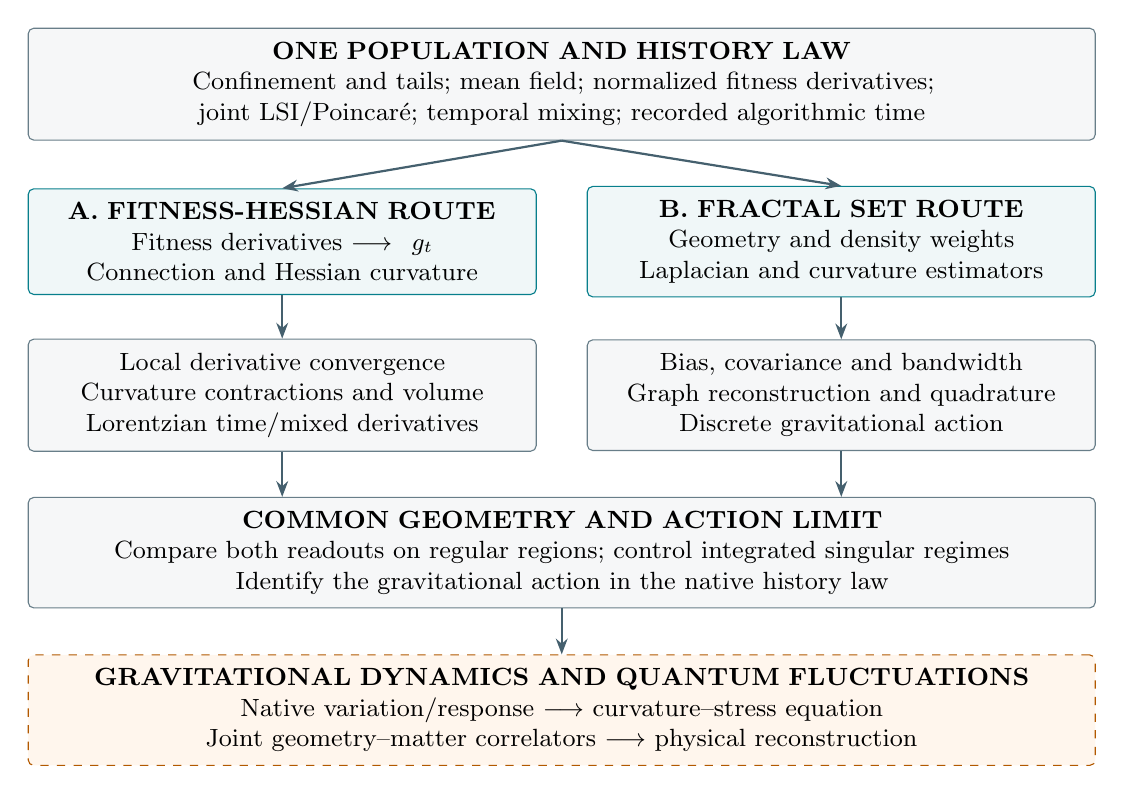
\begin{tikzpicture}[
 x=1cm,y=1cm,
 every node/.style={align=center,font=\small},
 qbox/.style={draw=ink!65,fill=ink!4,rounded corners=2pt,
 text width=6.1cm,minimum height=1.2cm,inner sep=5pt},
 qwide/.style={qbox,text width=13.2cm},
 qcontrol/.style={qbox,draw=teal,fill=teal!6},
 qtarget/.style={qwide,draw=orange!70!black,fill=orange!7,dashed},
 qflow/.style={-{Stealth[length=2mm]},draw=ink!80,line width=.8pt}]
\node[qwide] (root) at (0,0) {\textbf{ONE POPULATION AND HISTORY LAW}\\
Confinement and tails; mean field; normalized fitness derivatives;\\
joint LSI/Poincar\'e; temporal mixing; recorded algorithmic time};
\node[qcontrol] (metric) at (-3.55,-2) {\textbf{A. FITNESS-HESSIAN ROUTE}\\
Fitness derivatives $\longrightarrow g_t$\\
Connection and Hessian curvature};
\node[qcontrol] (graph) at (3.55,-2) {\textbf{B. FRACTAL SET ROUTE}\\
Geometry and density weights\\
Laplacian and curvature estimators};
\node[qbox] (direct) at (-3.55,-3.95) {Local derivative convergence\\
Curvature contractions and volume\\
Lorentzian time/mixed derivatives};
\node[qbox] (discrete) at (3.55,-3.95) {Bias, covariance and bandwidth\\
Graph reconstruction and quadrature\\
Discrete gravitational action};
\node[qwide] (join) at (0,-5.95) {\textbf{COMMON GEOMETRY AND ACTION LIMIT}\\
Compare both readouts on regular regions; control integrated singular regimes\\
Identify the gravitational action in the native history law};
\node[qtarget] (law) at (0,-7.95) {\textbf{GRAVITATIONAL DYNAMICS AND QUANTUM FLUCTUATIONS}\\
Native variation/response $\longrightarrow$ curvature--stress equation\\
Joint geometry--matter correlators $\longrightarrow$ physical reconstruction};
\draw[qflow] (root.south) -- (metric.north);
\draw[qflow] (root.south) -- (graph.north);
\draw[qflow] (metric.south) -- (direct.north);
\draw[qflow] (graph.south) -- (discrete.north);
\draw[qflow] (direct.south) -- (join.north -| direct.south);
\draw[qflow] (discrete.south) -- (join.north -| discrete.south);
\draw[qflow] (join.south) -- (law.north);
\end{tikzpicture}
\end{center}
{\small Solid boxes collect constructions and analytic tools already developed
in the source, with their stated hypotheses. The dashed box gives the
gravitational and quantum assembly to establish.}

\clearpage
\subsection{Route A: curvature from the fitness Hessian}
\label{sec:gravity-hessian}

\paragraph{Metric and population limit.}
Stage~\ref{stage:9} differentiates the complete normalized fitness, including
the companion-law derivatives when an expected field is used. The normalized
mean-field integral theorem and smooth empirical-field convergence theorem
give the derivative transfer
\[
V_{\mathrm{fit},N}\longrightarrow V_{\mathrm{fit}}[\mu]
\quad\hbox{in }C^r(K)
\]
on compact query regions under their denominator, domination and
equicontinuity hypotheses, for fixed reconstruction parameters
\hyperref[src:thm-cinf-mean-field-integrals]{[R47]}, \hyperref[src:thm-cinf-empirical-field-convergence]{[R48]}.
For varying bandwidths and regularizers, carry their constants along the
declared scale schedule. Conditional sampled fields retain their donor
context; comparing them with an expected field also requires the corresponding
conditional fluctuation estimate.

On a smooth positive Hessian branch, define
\[
\Phi_N=V_{\mathrm{fit},N}+\tfrac12\epsilon_g|x|^2,
\qquad g_{N,ab}=\partial_a\partial_b\Phi_N.
\]
On each regular region use a spectral margin $g_N\succeq m_KI$ and the
established matrix estimates to pass inverses, noise factors and volume
densities to their limits. The executed positive-part branch is
$g_N=\epsilon_gI+(H_N)_+$; its general curvature calculation uses the
derivatives of that selected metric. Smooth spectral regions and justified
weak reconstructions carry their own regularity conditions
\hyperref[src:prop-geometry-clipped-metric]{[R49]}.

\paragraph{Curvature theorem and proof mechanism.}
Write $C_{abc}=\partial_a\partial_b\partial_c\Phi$. The Hessian-curvature
lemma proves
\[
\Gamma^a_{bc}=\tfrac12g^{ap}C_{pbc},\qquad
R_{abcd}=\tfrac14g^{pq}
 (C_{adp}C_{bcq}-C_{acp}C_{bdq})
\qquad \hyperref[src:lem-curvature-hessian-cancellation]{[R113]}.
\]
Symmetry cancels the fourth derivatives in the antisymmetrized connection
derivative. The remaining terms are products of third derivatives and the
inverse metric. Under the lemma's classical regularity hypotheses,
$C^3(K)$ convergence of the potentials and a common spectral margin therefore
give uniform convergence of these spatial curvature components and their
Ricci, scalar and Einstein contractions. This consequence follows by
substitution in the displayed formula. A constant positive Hessian gives a
flat spatial metric; curvature is controlled by its spatial variation.

\paragraph{Algorithmic time and coupled evolution.}
The spatial metric becomes part of a Lorentzian spacetime reconstruction,
with recorded $t_n=nh$. In the product model $G=-c^2dt^2+g_t$, spacetime
curvature also depends on temporal and mixed derivatives. Control these
through the actual metric increments and the interpolation used in the limit.
The conditional metric law and coupled-field theorem already give those
increments jointly with the population, mechanical balances, noise and history
\hyperref[src:thm-algorithmic-conditional-metric-law]{[R114]},
\hyperref[src:thm-algorithmic-coupled-field-system]{[R35]}.
Thus the gravitational reduction starts from a specified coupled evolution.

\paragraph{Route A output.}
The output is a controlled spatial curvature field, its volume density, and
a spacetime curvature field when the temporal reconstruction estimates hold.
For the spacetime metric use the distinct notation
$\mathsf E_{ab}[G]=\operatorname{Ric}_{ab}[G]-\tfrac12R[G]G_{ab}$.
The fitness metric supplies the geometric input to this Einstein tensor.

\clearpage
\subsection{Route B: curvature and action from the Fractal Set}
\label{sec:gravity-fractal-set}

\paragraph{Transfer the existing analytic control.}
The complete-record encoding transports the established Dirichlet form, LSI
and Poincar\'e constants to Fractal Set observables
\hyperref[src:prop-fractal-set-analytic-transfer]{[R54]}. The joint law and the transported form
remain those of the recorded experiment. Temporal observations use their
specified history law and mixing estimates. This is the same foundation used
by Stages~\ref{stage:10}, \ref{stage:14} and \ref{stage:15}.

\paragraph{Laplacian convergence.}
For $M$ spatial observations and length bandwidth $\varepsilon$, the
unnormalized kernel theorem identifies
\[
L_{M,\varepsilon}\phi\longrightarrow
\frac{m_2}{2}\bigl(\rho\Delta_g\phi
 +2\langle\nabla\rho,\nabla\phi\rangle_g\bigr).
\]
Density correction and row normalization give the geometric operator
\[
L^{\mathrm{corr}}_{M,\varepsilon}\phi(x)
\xrightarrow{\mathbb P}\Delta_g\phi(x)
\qquad \hyperref[src:thm-laplacian-convergence]{[R115]},
\hyperref[src:prop-density-corrected-limit]{[R98]}.
\]
The proof expands the weighted integrand in normal coordinates, uses radial
kernel moments, and controls sampling fluctuations. The joint Poincar\'e
route bounds variance by $C_*C_H/(M\varepsilon^{d+4})$. For an estimated
density the theorem retains its local relative-error requirement. Recorded
graph distances, omitted edges and weights enter an explicit reconstruction
comparison after the operator normalization.

The spacetime nonlocal-operator theorem similarly converges to $\Box_G$,
with a covariance route or a joint Poincar\'e route for fluctuations
\hyperref[src:thm-cst-fractal-dalembertian-consistency]{[R116]},
\hyperref[src:lem-cst-poincare-variance]{[R117]}. These operator results and the curvature
result below have their own calibrated observables and error estimates.

\paragraph{Scalar-curvature theorem and proof mechanism.}
The curved neighborhood expansion fixes $M_0^{(R)}$ and $M_R\ne0$ through
\[
\varepsilon^{-D}\int\kappa^R_{\varepsilon,p}\,d\mathrm{vol}_G
 =M_0^{(R)}+M_RR[G](p)\varepsilon^2+O(\varepsilon^3).
\]
With the geometric sampling weights, define
\[
\widehat R_{\mathrm{FG}}(p)=\frac1{M_R\varepsilon^2}
\left[\frac1{M\varepsilon^D}\sum_{i=1}^M
 W_{\mathrm{geo}}(Y_i)\kappa^R_{\varepsilon,p}(Y_i)-M_0^{(R)}\right].
\]
The conditional scalar-curvature theorem proves
\[
\mathbb E|\widehat R_{\mathrm{FG}}(p)-R[G](p)|^2
\le C_1\varepsilon^2+\frac{C_2}{M\varepsilon^{D+4}}
\qquad \hyperref[src:thm-fractal-gas-ricci]{[R118]}.
\]
The expectation uses the calibrated geometric volume expansion; the variance
uses the covariance estimate for this curvature observable. Choose
$\varepsilon\to0$ with $M\varepsilon^{D+4}\to\infty$ and controlled constants.
Approximate episode inputs retain their normalized reconstruction error.

\paragraph{Route B output.}
With uniform convergence on the support of a test function $\chi$ and the
weighted quadrature law, the same theorem gives
\[
S_{\mathrm{FG},\chi}=\frac1{2\kappa M}\sum_i
 W_{\mathrm{geo}}(Y_i)\chi(Y_i)\widehat R_{\mathrm{FG}}(Y_i)
\xrightarrow{\mathbb P}
\frac1{2\kappa}\int\chi R[G]\,d\mathrm{vol}_G.
\]
This supplies an Einstein--Hilbert bulk-action approximation. Volume terms,
boundary terms and source contributions are added with their own common-law
quadrature and variation estimates. Noncompact action integrals use the
confinement and uniform-integrability estimates of Stage~\ref{stage:3}.

\clearpage
\subsection{Compare both routes and derive the gravitational law}

\paragraph{Agreement on a common geometry.}
Evaluate both routes using the same metric reconstruction, spacetime clock,
sampling law and normalization. On a regular compact region $K$, Route A
produces $R_N^{A}$ and Route B produces $\widehat R_N^{B}$. Their established
convergence estimates give
\[
|R_N^{A}(p)-\widehat R_N^{B}(p)|
\le |R_N^{A}(p)-R[G](p)|
 +|\widehat R_N^{B}(p)-R[G](p)|.
\]
Uniform versions give the action comparison on $K$. Spatial scalar curvature
is compared with a spatial estimator; spacetime scalar curvature is compared
with its spacetime estimator. Small-loop holonomy supplies a further
tensor-curvature readout under its transport-comparison hypotheses
\hyperref[src:thm-riemann-scutoid]{[R66]}. The scalar estimator and holonomy measurements thus
have distinct roles in recovering the full curvature tensor.

\paragraph{A causal-set action option.}
The Benincasa--Dowker construction offers a retarded layer-count operator
whose continuum expression is $\Box_G-\tfrac12R[G]$. Applying it to the
constant field extracts scalar curvature. A discrete action follows by
summing these contributions. This is an additional action construction on
the recorded order, requiring the actual interval-count sampling law,
scale-dependent fluctuation control and boundary calibration.
The source's localized two-sided operator and this retarded operator are
compared by their kernels, causal orientation and normalization
\hyperref[src:rem-cst-bd-comparison]{[R119]}.
The relevant external results are
\href{https://arxiv.org/abs/1001.2725}{Benincasa--Dowker, \emph{The Scalar Curvature of a Causal Set}}
and
\href{https://arxiv.org/abs/2007.13192}{Machet--Wang, \emph{On the continuum limit of the Benincasa--Dowker--Glaser causal set action}}.
The latter calculates the mean continuum action for sprinkled causal diamonds,
including an Einstein--Hilbert bulk term and a codimension-two boundary term.
The Fractal Gas application supplies its own correlated-history estimates.

\paragraph{Gravitational assembly criterion.}
Stage~\ref{stage:12} constructs the native descriptor action and source
response from the executed history law. Identify its geometric sector, on the
chosen scales, with an effective action of the form
\[
S_{\mathrm{eff}}[G,\Psi]
 =\frac1{2\kappa}\int(R[G]-2\Lambda)\,d\mathrm{vol}_G
 +S_{\mathrm{matter}}[G,\Psi]+S_{\mathrm{corr}}[G,\Psi].
\]
Here $\Psi$ denotes the retained matter and gauge fields, and
$S_{\mathrm{corr}}$ retains the derived higher-order and eliminated-field
contributions. Control first variations along the declared admissible metric
family, boundary data and sources. In a regime where stationarity holds for
the required metric variations, define
\[
T_{ab}=-\frac{2}{\sqrt{|\det G|}}
 \frac{\delta S_{\mathrm{matter}}}{\delta G^{ab}},\qquad
\mathcal C_{ab}=-\frac{2\kappa}{\sqrt{|\det G|}}
 \frac{\delta S_{\mathrm{corr}}}{\delta G^{ab}}.
\]
The variational identity then reads
\[
\mathsf E_{ab}[G]+\Lambda G_{ab}=\kappa T_{ab}+\mathcal C_{ab}.
\]
This displayed equation is the completion target for the native-action
identification. Its classical Einstein regime is obtained when the correction
tensor vanishes or is controlled at the stated approximation order.
Restricted Hessian variations initially give the corresponding projected
identity; obtaining the full tensor identity requires variations that determine
all its components. An equivalent route derives the curvature--stress law
directly from the coupled metric and mechanical evolution with a controlled
reduction. The source terms and memory corrections come from that evolution.

\clearpage
\subsection{Singular limits, information geometry and quantum fluctuations}

\paragraph{Regular regions and singular regimes.}
On each compact regular region $K$, use local derivative, spectral and sampling
estimates, allowing their constants to deteriorate toward singular regions.
A fixed spectral floor protects the implemented inverse; changing it requires
tracking its noise and comparison costs. Confinement controls probability tails.
Global bounded curvature is a restriction for a regular regime.

Near a proposed singular set, use an exhaustion by regular regions and a
specified weak or integrated curvature/action formulation. Estimate the omitted
contributions at their actual scale; if a finite integrated limit is sought,
prove the necessary integrability or state the chosen renormalization.
These are explicit tasks in the singular-regime extension of both routes.
A black-hole horizon is identified through the causal escape structure of the
reconstructed spacetime. Metric degeneracy, a clipping transition and invariant
curvature blow-up are measured separately. Horizon regularity can be tested
using a suitable spacetime chart; see
\href{https://vo.ned.ipac.caltech.edu/level5/March01/Carroll3/Carroll7.html}{Carroll, \emph{Lecture Notes on General Relativity}, Chapter 7}.

\paragraph{Fisher and Ruppeiner descriptions of Route A.}
For a regular exponential family
\[
p_\eta(y)=\exp\{\eta^aT_a(y)-A(\eta)\}\,h(y),\qquad
g^{\mathrm F}_{ab}=\partial_a\partial_bA
 =\operatorname{Cov}_{p_\eta}(T_a,T_b),
\]
the log-partition Hessian is the Fisher metric: differentiating normalization
gives $\partial_aA=\mathbb E_\eta T_a$, then the covariance identity.
Ruppeiner geometry uses the negative entropy Hessian in thermodynamic state
coordinates. Identifying fitness with the appropriate thermodynamic potential,
coordinate map and normalization realizes the Hessian route in information
geometry. Establish these identifications for the chosen population model,
then reuse its curvature and action estimates. See
\href{https://doi.org/10.1103/RevModPhys.67.605}{Ruppeiner, \emph{Riemannian geometry in thermodynamic fluctuation theory}}.

\paragraph{Retain the quantum geometry.}
The quantum-gravity extension retains fluctuations of geometry and matter in
the same equilibrium history. Route A constructs derivative-based geometric
observables; Route B constructs their discrete operator and action readouts.
Introduce jointly sourced correlations on the common recorded law,
\[
\mathcal Z_{N,h}(J,K)=\mathbb E_{P_{N,h}^{\mathrm{hist}}}
 \exp\!\left(i\sum_\alpha J_\alpha O^{\mathrm{geom}}_\alpha
             +i\sum_\beta K_\beta O^{\mathrm{matter}}_\beta\right).
\]
Use the established fluctuation, mixing and uniform-integrability estimates
to extract a joint hierarchy. Curvature probes are smeared or regularized on
the declared scales, with their observable-gradient or covariance costs
included. Connected geometry--matter correlations retain the fluctuations
discarded by a deterministic mean metric. Classical stationarity describes
the corresponding effective regime; quantum reconstruction uses the full
hierarchy and its physical positivity, causal and symmetry criteria.

\paragraph{Completion tasks for the combined extension.}
Carry the derivative bounds through the scale family; establish the recorded
geometric sampling and curvature calibration; compare both action readouts;
identify the native action and its variation; control singular regions; and
reconstruct the physical joint hierarchy. Shared confinement, mean-field,
LSI/Poincar\'e and history tools support both routes.

\clearpage
\section{How the proved walker dynamics supply the field theory}
This section collects the identifications used throughout the chapters into one dependency chain. Its starting point is the complete history of the three-dimensional gas at the recorded times \(t_n=n\Delta t\).

\subsection{Probability law, invariant descriptors, and frame observables}
The empirical walker law is
\[
L_N=\frac1N\sum_{i=1}^N\delta_{(x_i,v_i,a_i)}.
\]
The direct field law instead retains the full specified observable descriptor \(\mathscr O\) of the complete history:
\[
\mu_{\rm dir}=\mathscr O_*\mathbb P_{\rm rec},\qquad
\langle f\rangle_{\rm dir}
=\mathbb E_{\mathbb P_{\rm rec}}f(\mathscr O(\mathcal F)).
\]
The direct three-color definition sets \(d=3\) and constructs its masked vector from the actual viscous force and velocity:
\[
\widetilde c_i^a=F_i^{{\rm visc},a}e^{i\kappa v_i^a},\qquad
c_i=m_i\frac{\widetilde c_i}{\max(\|\widetilde c_i\|,\delta_c)}.
\]
The Gram and complex determinant coordinates identify the common internal-frame orbit and preserve its invariant history correlations. Full coordinates and masks are retained before forming the particular frame averages. A full-rank internal anchor chart is one explicit inverse chart; the full orbit theorem also covers the rank-deficient strata.

At a recorded frame, the book distinguishes the valid-weight average and its fixed-normalization companion:
\[
\mathcal A_t(O)=\frac{\sum_Iw_Im_IO_I}{W_t},\qquad
\mathcal A_t^N(O)=\frac1N\sum_Iw_Im_IO_I
=\frac{W_t}{N}\mathcal A_t(O),\qquad W_t=\sum_Iw_Im_I,
\]
with the recorded zero-denominator convention. Each is an observable of the same full history and has its own specified correlator. The physical meaning is read from the chosen descriptor and its temporal law.

\subsection{The history correlations retain the algorithmic clock}
For the selected invariant law \(\pi\), the lossless record theorem supplies
\[
\widehat P_hU=UP_h,\qquad
\widehat L=ULU^{-1}
\]
on the stated domain. The finite-step history formula and frame-correlator identity then give all retained correlations under the actual cloning and kinetic update. Cloning remains part of the evolution. Projection to a few channels uses the derived memory or the prediction-complete descriptor. Burn-in changes the initial law toward equilibrium; field time continues to be the calibrated recorded observation time.

\subsection{Geometric integrals and fluctuations have derived normalizations}
For the selected sampling law \(q\,d\mathrm{vol}_g\), the inverse-density formula converts normalized samples into geometric integrals. The normalized \(C^n\) calculus controls their coefficient fields. Joint LSI gives the direct empirical-gradient variance estimate, and the covariance route gives the alternative temporal/sampling estimate.

The centered hierarchy uses \(\sqrt N\) scaling around the actual stationary expectation. Its distribution-valued compactness and moment bounds retain the collective fluctuation information. The native gauge hierarchy separately retains the complex color algebra and its sourced history law. These constructions supply the background, fluctuations, and gauge correlations as distinct derived objects.

\subsection{Native likelihood and conditional geometry}
Condition the complete path likelihood on the descriptor and take its negative logarithm. This yields the field action, predictive kernel, and generating functional. The native source identities differentiate the executed update, and geometry-fiber disintegration preserves the conditional denominator. Recombination therefore returns the same sourced correlations. The continuum comparison uses the derived spatial geometry and the recorded time slices.

\subsection{Equilibrium representation and the gap}
The source specifies quantum reconstruction through the equilibrium temporal hierarchy and its stated physical representation hypotheses. The resulting transfer Hamiltonian uses that clock and observable law. The mass-gap passage then applies the proved self-adjoint gap-survival theorem with its uniform bound, embeddings, vacuum limit, and strong semigroup convergence.

\begin{criterion}[End-to-end composition]
For the configured \(3+1\) recorded family, apply the existing moment, population, regularity, sampling, and native-hierarchy results under their stated hypotheses. Identify its limiting equilibrium hierarchy with the physical Yang--Mills representation using the source's field-axiom and positive-transfer hypotheses. If the resulting Hamiltonians satisfy the uniform gap and convergence hypotheses of the gap-survival theorem, then
\[
\Spec(H)\subset\{0\}\cup[\lambda_*,\infty),\qquad
\ker H=\mathbb C\Omega,\qquad\lambda_*>0.
\]
The calibrated energy gap is at least \(\hbar_{\rm eff}\lambda_*\).
\end{criterion}
The criterion composes the source results. Representation hypotheses remain in their statements, while the population dynamics, normalizations, field equations, and inherited correlations are the constructions already derived in the chapters.

\clearpage
\section{The estimates that control the continuum}
\small
\begin{longtable}{@{}>{\raggedright\arraybackslash}p{.23\textwidth}>{\raggedright\arraybackslash}p{.35\textwidth}>{\raggedright\arraybackslash}p{.35\textwidth}@{}}
\toprule Tool & Controlled quantity & Constant or identification retained\\\midrule\endhead
Moment and tail drift & Escape, tightness, uniform integrability & Moment order, drift coefficient, coverage defect\\
Poincar\'e inequality & Empirical variance and form coercivity & Joint-law \(C_*\), appropriate Dirichlet form\\
Joint LSI & Entropy, concentration, fluctuation moments & Full gradient, status term, law identification\\
Hypocoercivity & Kinetic relaxation & Modified norm, prefactor, positive rate\\
Population comparison & Particle and time approximation & Initial moments, bias, horizon, attraction branch\\
Normalized \(C^n\) calculus & Smooth reconstructed coefficients & Kernel widths, floors, denominator lower bound\\
Local kernel calculus & Differential-operator bias & Geometry, moments, normal-coordinate bounds\\
Covariance estimate & Shrinking-neighborhood variance & \(C_{\rm mix}/(M\varepsilon^{D+2})\)\\
Direct joint-LSI estimate & Continuum error for dependent smooth observations & \(C_*C_\nabla/(M\varepsilon^{D+4})\)\\
Sampling density correction & Geometric integration from probability samples & Actual \(q\), weight \(q^{-1}\), selected law\\
Recorded operator comparison & Actual graph reconstruction & Error after \(\varepsilon^{-D-2}\) normalization\\
Temporal and ensemble perturbation & Weak, stationary, conditioned errors & Stability, resolvent rate, survival weights\\
Native likelihood and source identities & Gauge action and correlations & Descriptor support, geometry-fiber normalization\\
Physical reflection and symmetry & Quantum Hilbert space and dynamics & Selected spacetime hierarchy and physical clock\\
Strong semigroup convergence & Survival of a positive gap & \(J_a\), \(\Omega_a\), cutoff/volume-uniform \(\lambda_*\)\\
\bottomrule
\end{longtable}
\normalsize
\paragraph{Joint scale choice.}
Fix the transition parameters for each declared family, choose its observation regime using the population/time estimates, and set a bandwidth for which the local bias and correlated variance vanish. Then control reconstruction and action quadrature at that normalization. If \(h\), algorithmic locality, confinement, or noise changes, retain the corresponding uniform estimates for that changed transition family. Finally pass the sourced hierarchy and physical transfer operators through the same cutoff and volume sequence.

\clearpage
\appendix
\section{Source theorem register}
The references below point to the full statements and proofs in the repository snapshot. File paths are relative to \texttt{docs/source/2\_fractal\_gas/}. Line numbers identify the start of the named directive. The labels provide stable search keys when line numbers change.

\par\medskip\noindent\begin{minipage}{\linewidth}\textbf{[R1] Kinetic Gibbs reference measure}\label{src:def-gibbs-kinetic}\par
{\small\texttt{\detokenize{def-gibbs-kinetic}}\par
\nolinkurl{convergence_program/15_kl_convergence.md}, line 492.\par}
\end{minipage}\par

\par\medskip\noindent\begin{minipage}{\linewidth}\textbf{[R2] LSI for the kinetic reference measure}\label{src:thm-kinetic-lsi}\par
{\small\texttt{\detokenize{thm-kinetic-lsi}}\par
\nolinkurl{convergence_program/15_kl_convergence.md}, line 513.\par}
\end{minipage}\par

\par\medskip\noindent\begin{minipage}{\linewidth}\textbf{[R3] Identifying and testing a Gibbs QSD candidate}\label{src:thm-qsd-gibbs}\par
{\small\texttt{\detokenize{thm-qsd-gibbs}}\par
\nolinkurl{3_fitness_manifold/05_holography.md}, line 645.\par}
\end{minipage}\par

\par\medskip\noindent\begin{minipage}{\linewidth}\textbf{[R4] A normalized interaction with an explicit curvature bound}\label{src:prop-kl-joint-interaction-curvature}\par
{\small\texttt{\detokenize{prop-kl-joint-interaction-curvature}}\par
\nolinkurl{convergence_program/15_kl_convergence.md}, line 571.\par}
\end{minipage}\par

\par\medskip\noindent\begin{minipage}{\linewidth}\textbf{[R5] \(N\)-uniform LSI for specified joint laws}\label{src:cor-n-uniform-lsi}\par
{\small\texttt{\detokenize{cor-n-uniform-lsi}}\par
\nolinkurl{convergence_program/15_kl_convergence.md}, line 544.\par}
\end{minipage}\par

\par\medskip\noindent\begin{minipage}{\linewidth}\textbf{[R6] Poincaré inequality and empirical observables}\label{src:cor-quantitative-lsi-final}\par
{\small\texttt{\detokenize{cor-quantitative-lsi-final}}\par
\nolinkurl{convergence_program/15_kl_convergence.md}, line 2149.\par}
\end{minipage}\par

\par\medskip\noindent\begin{minipage}{\linewidth}\textbf{[R7] Kinetic and cloning convergence with a common target}\label{src:thm-main-kl-convergence}\par
{\small\texttt{\detokenize{thm-main-kl-convergence}}\par
\nolinkurl{convergence_program/15_kl_convergence.md}, line 1102.\par}
\end{minipage}\par

\par\medskip\noindent\begin{minipage}{\linewidth}\textbf{[R8] Entropy convergence for the full normalized swarm evolution}\label{src:thm-kl-convergence-euclidean}\par
{\small\texttt{\detokenize{thm-kl-convergence-euclidean}}\par
\nolinkurl{convergence_program/15_kl_convergence.md}, line 1164.\par}
\end{minipage}\par

\par\medskip\noindent\begin{minipage}{\linewidth}\textbf{[R9] Convergence of macroscopic observables}\label{src:thm-thermodynamic-limit}\par
{\small\texttt{\detokenize{thm-thermodynamic-limit}}\par
\nolinkurl{convergence_program/09_propagation_chaos.md}, line 4112.\par}
\end{minipage}\par

\par\medskip\noindent\begin{minipage}{\linewidth}\textbf{[R10] LSI for fixed marginals and their limits}\label{src:cor-kl-lsi-mean-field-limit}\par
{\small\texttt{\detokenize{cor-kl-lsi-mean-field-limit}}\par
\nolinkurl{convergence_program/15_kl_convergence.md}, line 2177.\par}
\end{minipage}\par

\par\medskip\noindent\begin{minipage}{\linewidth}\textbf{[R11] Algorithmic Evolution of Frame-Averaged Twistor Channels}\label{src:thm-effective-twistor-spectral-meaning}\par
{\small\texttt{\detokenize{thm-effective-twistor-spectral-meaning}}\par
\nolinkurl{2_fractal_set/08_twistor_formulation.md}, line 854.\par}
\end{minipage}\par

\par\medskip\noindent\begin{minipage}{\linewidth}\textbf{[R12] Action emergence from the recorded stochastic dynamics}\label{src:thm-ym-recorded-action-emergence}\par
{\small\texttt{\detokenize{thm-ym-recorded-action-emergence}}\par
\nolinkurl{2_fractal_set/05_yang_mills_noether.md}, line 321.\par}
\end{minipage}\par

\par\medskip\noindent\begin{minipage}{\linewidth}\textbf{[R13] Exact action on the recorded geometry fibers}\label{src:thm-ym-native-geometry-fiber-action}\par
{\small\texttt{\detokenize{thm-ym-native-geometry-fiber-action}}\par
\nolinkurl{2_fractal_set/05_yang_mills_noether.md}, line 3714.\par}
\end{minipage}\par

\par\medskip\noindent\begin{minipage}{\linewidth}\textbf{[R14] Static fluctuation-response identity for an exponential tilt}\label{src:prop-fluctuation-dissipation}\par
{\small\texttt{\detokenize{prop-fluctuation-dissipation}}\par
\nolinkurl{3_fitness_manifold/05_holography.md}, line 681.\par}
\end{minipage}\par

\par\medskip\noindent\begin{minipage}{\linewidth}\textbf{[R15] Stationary response from a discrete Poisson equation}\label{src:thm-algorithmic-stationary-response}\par
{\small\texttt{\detokenize{thm-algorithmic-stationary-response}}\par
\nolinkurl{3_fitness_manifold/05_holography.md}, line 873.\par}
\end{minipage}\par

\par\medskip\noindent\begin{minipage}{\linewidth}\textbf{[R16] Positive Transfer Representation of a Frame Correlator}\label{src:cor-effective-twistor-positive-transfer}\par
{\small\texttt{\detokenize{cor-effective-twistor-positive-transfer}}\par
\nolinkurl{2_fractal_set/08_twistor_formulation.md}, line 914.\par}
\end{minipage}\par

\par\medskip\noindent\begin{minipage}{\linewidth}\textbf{[R17] Survival of a uniformly controlled self-adjoint gap}\label{src:thm-mass-gap-rg-fixed-point}\par
{\small\texttt{\detokenize{thm-mass-gap-rg-fixed-point}}\par
\nolinkurl{2_fractal_set/05_yang_mills_noether.md}, line 5225.\par}
\end{minipage}\par

\par\medskip\noindent\begin{minipage}{\linewidth}\textbf{[R18] Component momentum, energy, and shared covariance}\label{src:thm-mean-field-component-identities}\par
{\small\texttt{\detokenize{thm-mean-field-component-identities}}\par
\nolinkurl{convergence_program/08_mean_field.md}, line 253.\par}
\end{minipage}\par

\par\medskip\noindent\begin{minipage}{\linewidth}\textbf{[R19] One-step collision consistency}\label{src:thm-mean-field-one-step-consistency}\par
{\small\texttt{\detokenize{thm-mean-field-one-step-consistency}}\par
\nolinkurl{convergence_program/08_mean_field.md}, line 278.\par}
\end{minipage}\par

\par\medskip\noindent\begin{minipage}{\linewidth}\textbf{[R20] Foster-Lyapunov drift for the composed kernel}\label{src:thm-foster-lyapunov-main}\par
{\small\texttt{\detokenize{thm-foster-lyapunov-main}}\par
\nolinkurl{convergence_program/06_convergence.md}, line 451.\par}
\end{minipage}\par

\par\medskip\noindent\begin{minipage}{\linewidth}\textbf{[R21] Fully evaluated selection-driven moment drift without a prescribed restoring trap}\label{src:thm-slceg-full-moment}\par
{\small\texttt{\detokenize{thm-slceg-full-moment}}\par
\nolinkurl{convergence_program/06a_structural_landscape_convergence.md}, line 15018.\par}
\end{minipage}\par

\par\medskip\noindent\begin{minipage}{\linewidth}\textbf{[R22] Entropy contraction to an explicit confinement floor}\label{src:thm-slce-entropy-floor}\par
{\small\texttt{\detokenize{thm-slce-entropy-floor}}\par
\nolinkurl{convergence_program/06a_structural_landscape_convergence.md}, line 15296.\par}
\end{minipage}\par

\par\medskip\noindent\begin{minipage}{\linewidth}\textbf{[R23] Structural/Barycenter Split for Full \(W_2\)}\label{src:thm-full-w2-split}\par
{\small\texttt{\detokenize{thm-full-w2-split}}\par
\nolinkurl{convergence_program/04_wasserstein_contraction.md}, line 560.\par}
\end{minipage}\par

\par\medskip\noindent\begin{minipage}{\linewidth}\textbf{[R24] Joint convergence of mass and shape}\label{src:thm-hk-convergence-main-assembly}\par
{\small\texttt{\detokenize{thm-hk-convergence-main-assembly}}\par
\nolinkurl{convergence_program/11_hk_convergence.md}, line 373.\par}
\end{minipage}\par

\par\medskip\noindent\begin{minipage}{\linewidth}\textbf{[R25] Finite-horizon survival from safe-walker estimates}\label{src:thm-exponential-survival}\par
{\small\texttt{\detokenize{thm-exponential-survival}}\par
\nolinkurl{convergence_program/11_hk_convergence.md}, line 245.\par}
\end{minipage}\par

\par\medskip\noindent\begin{minipage}{\linewidth}\textbf{[R26] A weighted coupling form of Harris' argument}\label{src:thm-convergence-conservative-harris}\par
{\small\texttt{\detokenize{thm-convergence-conservative-harris}}\par
\nolinkurl{convergence_program/06_convergence.md}, line 649.\par}
\end{minipage}\par

\par\medskip\noindent\begin{minipage}{\linewidth}\textbf{[R27] QSD convergence from a two-sided surviving-block bound}\label{src:thm-main-convergence}\par
{\small\texttt{\detokenize{thm-main-convergence}}\par
\nolinkurl{convergence_program/06_convergence.md}, line 801.\par}
\end{minipage}\par

\par\medskip\noindent\begin{minipage}{\linewidth}\textbf{[R28] Relaxation to the selected law of a recorded gauge window}\label{src:thm-ym-qsd-window-relaxation}\par
{\small\texttt{\detokenize{thm-ym-qsd-window-relaxation}}\par
\nolinkurl{2_fractal_set/05_yang_mills_noether.md}, line 6228.\par}
\end{minipage}\par

\par\medskip\noindent\begin{minipage}{\linewidth}\textbf{[R29] The fixed-step mean-field equation}\label{src:thm-mean-field-equation}\par
{\small\texttt{\detokenize{thm-mean-field-equation}}\par
\nolinkurl{convergence_program/08_mean_field.md}, line 395.\par}
\end{minipage}\par

\par\medskip\noindent\begin{minipage}{\linewidth}\textbf{[R30] Exact mass and weak field balances}\label{src:thm-mass-conservation}\par
{\small\texttt{\detokenize{thm-mass-conservation}}\par
\nolinkurl{convergence_program/08_mean_field.md}, line 422.\par}
\end{minipage}\par

\par\medskip\noindent\begin{minipage}{\linewidth}\textbf{[R31] Explicit finite-step population law}\label{src:thm-algorithmic-explicit-transition}\par
{\small\texttt{\detokenize{thm-algorithmic-explicit-transition}}\par
\nolinkurl{3_fitness_manifold/04_field_equations.md}, line 230.\par}
\end{minipage}\par

\par\medskip\noindent\begin{minipage}{\linewidth}\textbf{[R32] Exact field characteristics and moment hierarchy}\label{src:thm-algorithmic-field-characteristics}\par
{\small\texttt{\detokenize{thm-algorithmic-field-characteristics}}\par
\nolinkurl{3_fitness_manifold/04_field_equations.md}, line 282.\par}
\end{minipage}\par

\par\medskip\noindent\begin{minipage}{\linewidth}\textbf{[R33] Finite-step observable equation and fluctuation covariance}\label{src:thm-algorithmic-observable-increment}\par
{\small\texttt{\detokenize{thm-algorithmic-observable-increment}}\par
\nolinkurl{3_fitness_manifold/04_field_equations.md}, line 657.\par}
\end{minipage}\par

\par\medskip\noindent\begin{minipage}{\linewidth}\textbf{[R34] Exact discrete spatial density and momentum equations}\label{src:thm-algorithmic-spatial-field-equations}\par
{\small\texttt{\detokenize{thm-algorithmic-spatial-field-equations}}\par
\nolinkurl{3_fitness_manifold/04_field_equations.md}, line 1899.\par}
\end{minipage}\par

\par\medskip\noindent\begin{minipage}{\linewidth}\textbf{[R35] Coupled population, mechanical, and metric fields}\label{src:thm-algorithmic-coupled-field-system}\par
{\small\texttt{\detokenize{thm-algorithmic-coupled-field-system}}\par
\nolinkurl{3_fitness_manifold/04_field_equations.md}, line 2106.\par}
\end{minipage}\par

\par\medskip\noindent\begin{minipage}{\linewidth}\textbf{[R36] Finite-horizon propagation of chaos for the actual update}\label{src:thm-chaos-finite-time-consistency}\par
{\small\texttt{\detokenize{thm-chaos-finite-time-consistency}}\par
\nolinkurl{convergence_program/09_propagation_chaos.md}, line 1190.\par}
\end{minipage}\par

\par\medskip\noindent\begin{minipage}{\linewidth}\textbf{[R37] Closed full-law convergence with unbounded raw reward}\label{src:thm-slcw-active-contraction}\par
{\small\texttt{\detokenize{thm-slcw-active-contraction}}\par
\nolinkurl{convergence_program/06a_structural_landscape_convergence.md}, line 14371.\par}
\end{minipage}\par

\par\medskip\noindent\begin{minipage}{\linewidth}\textbf{[R38] Uniform-time trajectories, stationary chaos and commuting limits}\label{src:cor-slcw-trajectories}\par
{\small\texttt{\detokenize{cor-slcw-trajectories}}\par
\nolinkurl{convergence_program/06a_structural_landscape_convergence.md}, line 14710.\par}
\end{minipage}\par

\par\medskip\noindent\begin{minipage}{\linewidth}\textbf{[R39] Uniform trajectory approximation through a diverging horizon}\label{src:thm-slcgt-growing-trajectory}\par
{\small\texttt{\detokenize{thm-slcgt-growing-trajectory}}\par
\nolinkurl{convergence_program/06a_structural_landscape_convergence.md}, line 18248.\par}
\end{minipage}\par

\par\medskip\noindent\begin{minipage}{\linewidth}\textbf{[R40] Exchangeability of a unique QSD}\label{src:thm-qsd-exchangeability}\par
{\small\texttt{\detokenize{thm-qsd-exchangeability}}\par
\nolinkurl{convergence_program/12_qsd_exchangeability_theory.md}, line 37.\par}
\end{minipage}\par

\par\medskip\noindent\begin{minipage}{\linewidth}\textbf{[R41] Deterministic empirical limits imply chaos}\label{src:thm-propagation-chaos-qsd}\par
{\small\texttt{\detokenize{thm-propagation-chaos-qsd}}\par
\nolinkurl{convergence_program/12_qsd_exchangeability_theory.md}, line 181.\par}
\end{minipage}\par

\par\medskip\noindent\begin{minipage}{\linewidth}\textbf{[R42] Exact covariance identity for finite populations}\label{src:thm-correlation-decay}\par
{\small\texttt{\detokenize{thm-correlation-decay}}\par
\nolinkurl{convergence_program/12_qsd_exchangeability_theory.md}, line 212.\par}
\end{minipage}\par

\par\medskip\noindent\begin{minipage}{\linewidth}\textbf{[R43] LSI from a quadratic Lyapunov bound}\label{src:thm-unconditional-lsi}\par
{\small\texttt{\detokenize{thm-unconditional-lsi}}\par
\nolinkurl{convergence_program/15_kl_convergence.md}, line 369.\par}
\end{minipage}\par

\par\medskip\noindent\begin{minipage}{\linewidth}\textbf{[R44] Kinetic hypocoercive entropy convergence}\label{src:thm-villani-hypocoercivity}\par
{\small\texttt{\detokenize{thm-villani-hypocoercivity}}\par
\nolinkurl{convergence_program/15_kl_convergence.md}, line 805.\par}
\end{minipage}\par

\par\medskip\noindent\begin{minipage}{\linewidth}\textbf{[R45] C³ regularity of sampled, surrogate, and expected fitness}\label{src:thm-c3-regularity}\par
{\small\texttt{\detokenize{thm-c3-regularity}}\par
\nolinkurl{convergence_program/14_a_geometric_gas_c3_regularity.md}, line 726.\par}
\end{minipage}\par

\par\medskip\noindent\begin{minipage}{\linewidth}\textbf{[R46] Full sampled-fitness majorant}\label{src:thm-main-cinf-regularity-fitness-potential-full}\par
{\small\texttt{\detokenize{thm-main-cinf-regularity-fitness-potential-full}}\par
\nolinkurl{convergence_program/14_b_geometric_gas_cinf_regularity_full.md}, line 963.\par}
\end{minipage}\par

\par\medskip\noindent\begin{minipage}{\linewidth}\textbf{[R47] Differentiating normalized mean-field integrals}\label{src:thm-cinf-mean-field-integrals}\par
{\small\texttt{\detokenize{thm-cinf-mean-field-integrals}}\par
\nolinkurl{convergence_program/14_b_geometric_gas_cinf_regularity_full.md}, line 1396.\par}
\end{minipage}\par

\par\medskip\noindent\begin{minipage}{\linewidth}\textbf{[R48] Smooth convergence of normalized empirical fields}\label{src:thm-cinf-empirical-field-convergence}\par
{\small\texttt{\detokenize{thm-cinf-empirical-field-convergence}}\par
\nolinkurl{convergence_program/14_b_geometric_gas_cinf_regularity_full.md}, line 1426.\par}
\end{minipage}\par

\par\medskip\noindent\begin{minipage}{\linewidth}\textbf{[R49] Metric represented by the implemented Hessian branch}\label{src:prop-geometry-clipped-metric}\par
{\small\texttt{\detokenize{prop-geometry-clipped-metric}}\par
\nolinkurl{3_fitness_manifold/01_emergent_geometry.md}, line 122.\par}
\end{minipage}\par

\par\medskip\noindent\begin{minipage}{\linewidth}\textbf{[R50] Uniform ellipticity from metric bounds}\label{src:thm-uniform-ellipticity-latent}\par
{\small\texttt{\detokenize{thm-uniform-ellipticity-latent}}\par
\nolinkurl{3_fitness_manifold/01_emergent_geometry.md}, line 234.\par}
\end{minipage}\par

\par\medskip\noindent\begin{minipage}{\linewidth}\textbf{[R51] Uniform ellipticity from the spectral margin}\label{src:thm-gg-ueph-construction}\par
{\small\texttt{\detokenize{thm-gg-ueph-construction}}\par
\nolinkurl{convergence_program/17_geometric_gas.md}, line 197.\par}
\end{minipage}\par

\par\medskip\noindent\begin{minipage}{\linewidth}\textbf{[R52] \(N\)-uniform LSI for an identified geometric law}\label{src:thm-gg-lsi-main}\par
{\small\texttt{\detokenize{thm-gg-lsi-main}}\par
\nolinkurl{convergence_program/17_geometric_gas.md}, line 720.\par}
\end{minipage}\par

\par\medskip\noindent\begin{minipage}{\linewidth}\textbf{[R53] Lossless Reconstruction}\label{src:thm-fractal-set-lossless}\par
{\small\texttt{\detokenize{thm-fractal-set-lossless}}\par
\nolinkurl{2_fractal_set/01_fractal_set.md}, line 1638.\par}
\end{minipage}\par

\par\medskip\noindent\begin{minipage}{\linewidth}\textbf{[R54] Transport of record observables and established estimates}\label{src:prop-fractal-set-analytic-transfer}\par
{\small\texttt{\detokenize{prop-fractal-set-analytic-transfer}}\par
\nolinkurl{2_fractal_set/01_fractal_set.md}, line 1955.\par}
\end{minipage}\par

\par\medskip\noindent\begin{minipage}{\linewidth}\textbf{[R55] Measure and observable isomorphism for invariant coordinates}\label{src:thm-sm-direct-measure-isomorphism}\par
{\small\texttt{\detokenize{thm-sm-direct-measure-isomorphism}}\par
\nolinkurl{2_fractal_set/04_standard_model.md}, line 1759.\par}
\end{minipage}\par

\par\medskip\noindent\begin{minipage}{\linewidth}\textbf{[R56] Exact transition and history isomorphism for the recorded algorithm}\label{src:thm-sm-instantiated-record-transition}\par
{\small\texttt{\detokenize{thm-sm-instantiated-record-transition}}\par
\nolinkurl{2_fractal_set/04_standard_model.md}, line 2736.\par}
\end{minipage}\par

\par\medskip\noindent\begin{minipage}{\linewidth}\textbf{[R57] The recorded Fractal Set is a causal set}\label{src:thm-fractal-is-causal-set}\par
{\small\texttt{\detokenize{thm-fractal-is-causal-set}}\par
\nolinkurl{2_fractal_set/02_causal_set_theory.md}, line 131.\par}
\end{minipage}\par

\par\medskip\noindent\begin{minipage}{\linewidth}\textbf{[R58] Conditional compatibility of CST paths and geometric causality}\label{src:prop-fractal-causal-order-equivalence}\par
{\small\texttt{\detokenize{prop-fractal-causal-order-equivalence}}\par
\nolinkurl{2_fractal_set/02_causal_set_theory.md}, line 237.\par}
\end{minipage}\par

\par\medskip\noindent\begin{minipage}{\linewidth}\textbf{[R59] Conditional volume matching and trajectory clocks}\label{src:thm-fractal-faithful-embedding}\par
{\small\texttt{\detokenize{thm-fractal-faithful-embedding}}\par
\nolinkurl{2_fractal_set/02_causal_set_theory.md}, line 616.\par}
\end{minipage}\par

\par\medskip\noindent\begin{minipage}{\linewidth}\textbf{[R60] Slab consistency and the scope of causal convergence}\label{src:prop-scutoid-cst-compatibility}\par
{\small\texttt{\detokenize{prop-scutoid-cst-compatibility}}\par
\nolinkurl{3_fitness_manifold/02_scutoid_spacetime.md}, line 483.\par}
\end{minipage}\par

\par\medskip\noindent\begin{minipage}{\linewidth}\textbf{[R61] Gram and determinant coordinates for SU(n) orbits}\label{src:thm-sm-direct-orbit-isomorphism}\par
{\small\texttt{\detokenize{thm-sm-direct-orbit-isomorphism}}\par
\nolinkurl{2_fractal_set/04_standard_model.md}, line 1542.\par}
\end{minipage}\par

\par\medskip\noindent\begin{minipage}{\linewidth}\textbf{[R62] SU(2) from Hermitian and alternating doublet contractions}\label{src:thm-sm-direct-su2-invariants}\par
{\small\texttt{\detokenize{thm-sm-direct-su2-invariants}}\par
\nolinkurl{2_fractal_set/04_standard_model.md}, line 1270.\par}
\end{minipage}\par

\par\medskip\noindent\begin{minipage}{\linewidth}\textbf{[R63] Interaction holonomy and angular matter energy of the recorded connection}\label{src:prop-ym-recorded-interaction-sector}\par
{\small\texttt{\detokenize{prop-ym-recorded-interaction-sector}}\par
\nolinkurl{2_fractal_set/05_yang_mills_noether.md}, line 605.\par}
\end{minipage}\par

\par\medskip\noindent\begin{minipage}{\linewidth}\textbf{[R64] Gauge invariance of Wilson observables and actions}\label{src:thm-wilson-action-gauge-invariance}\par
{\small\texttt{\detokenize{thm-wilson-action-gauge-invariance}}\par
\nolinkurl{2_fractal_set/05_yang_mills_noether.md}, line 1649.\par}
\end{minipage}\par

\par\medskip\noindent\begin{minipage}{\linewidth}\textbf{[R65] Error accumulation for comparison holonomy}\label{src:lem-regge-holonomy-approx}\par
{\small\texttt{\detokenize{lem-regge-holonomy-approx}}\par
\nolinkurl{3_fitness_manifold/03_curvature_gravity.md}, line 955.\par}
\end{minipage}\par

\par\medskip\noindent\begin{minipage}{\linewidth}\textbf{[R66] Curvature recovery from consistent plaquette transport}\label{src:thm-riemann-scutoid}\par
{\small\texttt{\detokenize{thm-riemann-scutoid}}\par
\nolinkurl{3_fitness_manifold/03_curvature_gravity.md}, line 991.\par}
\end{minipage}\par

\par\medskip\noindent\begin{minipage}{\linewidth}\textbf{[R67] Quantitative curvature expansion of the recorded face action}\label{src:lem-ym-recorded-face-action-remainder}\par
{\small\texttt{\detokenize{lem-ym-recorded-face-action-remainder}}\par
\nolinkurl{2_fractal_set/05_yang_mills_noether.md}, line 507.\par}
\end{minipage}\par

\par\medskip\noindent\begin{minipage}{\linewidth}\textbf{[R68] Reference-transport covariance}\label{src:lem-reference-transport-covariance}\par
{\small\texttt{\detokenize{lem-reference-transport-covariance}}\par
\nolinkurl{3_fitness_manifold/09_measurement.md}, line 627.\par}
\end{minipage}\par

\par\medskip\noindent\begin{minipage}{\linewidth}\textbf{[R69] Effective gauge-channel action and predictive kernel of the recorded algorithm}\label{src:thm-sm-effective-recorded-gauge-dynamics}\par
{\small\texttt{\detokenize{thm-sm-effective-recorded-gauge-dynamics}}\par
\nolinkurl{2_fractal_set/04_standard_model.md}, line 4020.\par}
\end{minipage}\par

\par\medskip\noindent\begin{minipage}{\linewidth}\textbf{[R70] Exact source response of the algorithm-derived field action}\label{src:thm-ym-native-source-response}\par
{\small\texttt{\detokenize{thm-ym-native-source-response}}\par
\nolinkurl{2_fractal_set/05_yang_mills_noether.md}, line 1686.\par}
\end{minipage}\par

\par\medskip\noindent\begin{minipage}{\linewidth}\textbf{[R71] Transient projected field equation}\label{src:thm-algorithmic-transient-field-memory}\par
{\small\texttt{\detokenize{thm-algorithmic-transient-field-memory}}\par
\nolinkurl{3_fitness_manifold/04_field_equations.md}, line 1641.\par}
\end{minipage}\par

\par\medskip\noindent\begin{minipage}{\linewidth}\textbf{[R72] Field evolution conditional on its observed history}\label{src:thm-algorithmic-field-filter}\par
{\small\texttt{\detokenize{thm-algorithmic-field-filter}}\par
\nolinkurl{3_fitness_manifold/04_field_equations.md}, line 1768.\par}
\end{minipage}\par

\par\medskip\noindent\begin{minipage}{\linewidth}\textbf{[R73] Prediction-complete gauge descriptors from the actual transition}\label{src:thm-sm-prediction-complete-descriptors}\par
{\small\texttt{\detokenize{thm-sm-prediction-complete-descriptors}}\par
\nolinkurl{2_fractal_set/04_standard_model.md}, line 2083.\par}
\end{minipage}\par

\par\medskip\noindent\begin{minipage}{\linewidth}\textbf{[R74] Finite transition matrices converging to the completed channel theory}\label{src:thm-sm-predictive-partition-convergence}\par
{\small\texttt{\detokenize{thm-sm-predictive-partition-convergence}}\par
\nolinkurl{2_fractal_set/04_standard_model.md}, line 2201.\par}
\end{minipage}\par

\par\medskip\noindent\begin{minipage}{\linewidth}\textbf{[R75] Closure implications and their converse}\label{src:thm-closure-equivalence-cosmo}\par
{\small\texttt{\detokenize{thm-closure-equivalence-cosmo}}\par
\nolinkurl{3_fitness_manifold/06_cosmology.md}, line 351.\par}
\end{minipage}\par

\par\medskip\noindent\begin{minipage}{\linewidth}\textbf{[R76] Exact and approximate Markov closure}\label{src:prop-cosmo-generator-closure}\par
{\small\texttt{\detokenize{prop-cosmo-generator-closure}}\par
\nolinkurl{3_fitness_manifold/06_cosmology.md}, line 391.\par}
\end{minipage}\par

\par\medskip\noindent\begin{minipage}{\linewidth}\textbf{[R77] Exact path KL identities}\label{src:prop-algorithmic-path-kl-identities}\par
{\small\texttt{\detokenize{prop-algorithmic-path-kl-identities}}\par
\nolinkurl{3_fitness_manifold/05_holography.md}, line 797.\par}
\end{minipage}\par

\par\medskip\noindent\begin{minipage}{\linewidth}\textbf{[R78] Faithful exterior algebra of alternating recorded insertions}\label{src:thm-lqft-oriented-word-algebra}\par
{\small\texttt{\detokenize{thm-lqft-oriented-word-algebra}}\par
\nolinkurl{2_fractal_set/03_lattice_qft.md}, line 681.\par}
\end{minipage}\par

\par\medskip\noindent\begin{minipage}{\linewidth}\textbf{[R79] Completely positive CAR evolution of the recorded contraction}\label{src:thm-lqft-record-car-channel}\par
{\small\texttt{\detokenize{thm-lqft-record-car-channel}}\par
\nolinkurl{2_fractal_set/03_lattice_qft.md}, line 1018.\par}
\end{minipage}\par

\par\medskip\noindent\begin{minipage}{\linewidth}\textbf{[R80] Separate local-net application to the recorded CAR representation}\label{src:thm-ym-hk-record-instantiation}\par
{\small\texttt{\detokenize{thm-ym-hk-record-instantiation}}\par
\nolinkurl{2_fractal_set/05_yang_mills_noether.md}, line 9275.\par}
\end{minipage}\par

\par\medskip\noindent\begin{minipage}{\linewidth}\textbf{[R81] Native fermion evolution, localization, and record covariance}\label{src:thm-lqft-native-local-fermion-evolution}\par
{\small\texttt{\detokenize{thm-lqft-native-local-fermion-evolution}}\par
\nolinkurl{2_fractal_set/03_lattice_qft.md}, line 1585.\par}
\end{minipage}\par

\par\medskip\noindent\begin{minipage}{\linewidth}\textbf{[R82] Exact inherited-history covariance of native regional readouts}\label{src:thm-lqft-inherited-history-covariance}\par
{\small\texttt{\detokenize{thm-lqft-inherited-history-covariance}}\par
\nolinkurl{2_fractal_set/03_lattice_qft.md}, line 1332.\par}
\end{minipage}\par

\par\medskip\noindent\begin{minipage}{\linewidth}\textbf{[R83] Existing LSI and native contraction bounds}\label{src:cor-lqft-fock-lsi-transfer}\par
{\small\texttt{\detokenize{cor-lqft-fock-lsi-transfer}}\par
\nolinkurl{2_fractal_set/03_lattice_qft.md}, line 1186.\par}
\end{minipage}\par

\par\medskip\noindent\begin{minipage}{\linewidth}\textbf{[R84] Distribution-valued compactness from the established stationary LSI}\label{src:thm-ym-spacetime-fluctuation-compactness}\par
{\small\texttt{\detokenize{thm-ym-spacetime-fluctuation-compactness}}\par
\nolinkurl{2_fractal_set/05_yang_mills_noether.md}, line 5512.\par}
\end{minipage}\par

\par\medskip\noindent\begin{minipage}{\linewidth}\textbf{[R85] Drift and covariance equations for the complete selected update}\label{src:prop-ym-complete-fluctuation-equations}\par
{\small\texttt{\detokenize{prop-ym-complete-fluctuation-equations}}\par
\nolinkurl{2_fractal_set/05_yang_mills_noether.md}, line 5750.\par}
\end{minipage}\par

\par\medskip\noindent\begin{minipage}{\linewidth}\textbf{[R86] Native physical hierarchy of the full recorded color invariants}\label{src:thm-ym-native-physical-gauge-hierarchy}\par
{\small\texttt{\detokenize{thm-ym-native-physical-gauge-hierarchy}}\par
\nolinkurl{2_fractal_set/05_yang_mills_noether.md}, line 7629.\par}
\end{minipage}\par

\par\medskip\noindent\begin{minipage}{\linewidth}\textbf{[R87] Geometry-fiber action in the common native continuum limit}\label{src:thm-ym-native-fiber-continuum}\par
{\small\texttt{\detokenize{thm-ym-native-fiber-continuum}}\par
\nolinkurl{2_fractal_set/05_yang_mills_noether.md}, line 3914.\par}
\end{minipage}\par

\par\medskip\noindent\begin{minipage}{\linewidth}\textbf{[R88] Nontrivial doublet fluctuations from the actual companion draw}\label{src:thm-sm-native-doublet-fluctuations}\par
{\small\texttt{\detokenize{thm-sm-native-doublet-fluctuations}}\par
\nolinkurl{2_fractal_set/04_standard_model.md}, line 1087.\par}
\end{minipage}\par

\par\medskip\noindent\begin{minipage}{\linewidth}\textbf{[R89] Nonzero momentum fluctuations in the established Euclidean paired model}\label{src:cor-ym-paired-momentum-fluctuations}\par
{\small\texttt{\detokenize{cor-ym-paired-momentum-fluctuations}}\par
\nolinkurl{2_fractal_set/05_yang_mills_noether.md}, line 6405.\par}
\end{minipage}\par

\par\medskip\noindent\begin{minipage}{\linewidth}\textbf{[R90] Uniform integrability and reconstruction bounds for the full direct color algebra}\label{src:lem-ym-physical-gauge-word-uniform-integrability}\par
{\small\texttt{\detokenize{lem-ym-physical-gauge-word-uniform-integrability}}\par
\nolinkurl{2_fractal_set/05_yang_mills_noether.md}, line 7546.\par}
\end{minipage}\par

\par\medskip\noindent\begin{minipage}{\linewidth}\textbf{[R91] Direct local bias estimate in specified normal coordinates}\label{src:lem-continuum-local-bias}\par
{\small\texttt{\detokenize{lem-continuum-local-bias}}\par
\nolinkurl{convergence_program/16_continuum_discharge.md}, line 509.\par}
\end{minipage}\par

\par\medskip\noindent\begin{minipage}{\linewidth}\textbf{[R92] A covariance condition sufficient for A4}\label{src:lem-continuum-a4-mixing}\par
{\small\texttt{\detokenize{lem-continuum-a4-mixing}}\par
\nolinkurl{convergence_program/16_continuum_discharge.md}, line 597.\par}
\end{minipage}\par

\par\medskip\noindent\begin{minipage}{\linewidth}\textbf{[R93] A sufficient bandwidth schedule for A6}\label{src:lem-continuum-a6-scaling}\par
{\small\texttt{\detokenize{lem-continuum-a6-scaling}}\par
\nolinkurl{convergence_program/16_continuum_discharge.md}, line 687.\par}
\end{minipage}\par

\par\medskip\noindent\begin{minipage}{\linewidth}\textbf{[R94] Conditional continuum consistency}\label{src:cor-continuum-consistency-conditional}\par
{\small\texttt{\detokenize{cor-continuum-consistency-conditional}}\par
\nolinkurl{convergence_program/16_continuum_discharge.md}, line 735.\par}
\end{minipage}\par

\par\medskip\noindent\begin{minipage}{\linewidth}\textbf{[R95] Normalized sampling and the distinction between QSD and invariance}\label{src:lem-continuum-a3-qsd-sampling}\par
{\small\texttt{\detokenize{lem-continuum-a3-qsd-sampling}}\par
\nolinkurl{convergence_program/16_continuum_discharge.md}, line 327.\par}
\end{minipage}\par

\par\medskip\noindent\begin{minipage}{\linewidth}\textbf{[R96] Normalized importance sampling and variance}\label{src:prop-monte-carlo-riemannian-latent}\par
{\small\texttt{\detokenize{prop-monte-carlo-riemannian-latent}}\par
\nolinkurl{3_fitness_manifold/01_emergent_geometry.md}, line 1116.\par}
\end{minipage}\par

\par\medskip\noindent\begin{minipage}{\linewidth}\textbf{[R97] Continuum estimator error from the established joint LSI}\label{src:cor-cst-inherited-lsi-consistency}\par
{\small\texttt{\detokenize{cor-cst-inherited-lsi-consistency}}\par
\nolinkurl{2_fractal_set/02_causal_set_theory.md}, line 966.\par}
\end{minipage}\par

\par\medskip\noindent\begin{minipage}{\linewidth}\textbf{[R98] Density-corrected limit with sufficient sampling control}\label{src:prop-density-corrected-limit}\par
{\small\texttt{\detokenize{prop-density-corrected-limit}}\par
\nolinkurl{2_fractal_set/03_lattice_qft.md}, line 2185.\par}
\end{minipage}\par

\par\medskip\noindent\begin{minipage}{\linewidth}\textbf{[R99] Volume Element Transformation}\label{src:thm-volume-element-transformation}\par
{\small\texttt{\detokenize{thm-volume-element-transformation}}\par
\nolinkurl{3_fitness_manifold/07_computational_proxies.md}, line 1155.\par}
\end{minipage}\par

\par\medskip\noindent\begin{minipage}{\linewidth}\textbf{[R100] Wilson action consistency under geometric quadrature}\label{src:thm-continuum-limit-ym}\par
{\small\texttt{\detokenize{thm-continuum-limit-ym}}\par
\nolinkurl{2_fractal_set/05_yang_mills_noether.md}, line 4858.\par}
\end{minipage}\par

\par\medskip\noindent\begin{minipage}{\linewidth}\textbf{[R101] Common continuum limit of the native source likelihood and descriptor action}\label{src:thm-ym-continuum-source-action}\par
{\small\texttt{\detokenize{thm-ym-continuum-source-action}}\par
\nolinkurl{2_fractal_set/05_yang_mills_noether.md}, line 2714.\par}
\end{minipage}\par

\par\medskip\noindent\begin{minipage}{\linewidth}\textbf{[R102] Time consistency for the specified transition family}\label{src:thm-correct-continuum-limit}\par
{\small\texttt{\detokenize{thm-correct-continuum-limit}}\par
\nolinkurl{2_fractal_set/05_yang_mills_noether.md}, line 5180.\par}
\end{minipage}\par

\par\medskip\noindent\begin{minipage}{\linewidth}\textbf{[R103] Total observable error}\label{src:thm-total-error-bound}\par
{\small\texttt{\detokenize{thm-total-error-bound}}\par
\nolinkurl{convergence_program/13_quantitative_error_bounds.md}, line 719.\par}
\end{minipage}\par

\par\medskip\noindent\begin{minipage}{\linewidth}\textbf{[R104] Native response current in recorded spacetime}\label{src:thm-ym-native-response-current}\par
{\small\texttt{\detokenize{thm-ym-native-response-current}}\par
\nolinkurl{2_fractal_set/05_yang_mills_noether.md}, line 2376.\par}
\end{minipage}\par

\par\medskip\noindent\begin{minipage}{\linewidth}\textbf{[R105] Native response and the weak connection-variation identity}\label{src:prop-ym-native-connection-variation-identity}\par
{\small\texttt{\detokenize{prop-ym-native-connection-variation-identity}}\par
\nolinkurl{2_fractal_set/05_yang_mills_noether.md}, line 4158.\par}
\end{minipage}\par

\par\medskip\noindent\begin{minipage}{\linewidth}\textbf{[R106] Exact graph Ward identity}\label{src:lem-ym-discrete-ward}\par
{\small\texttt{\detokenize{lem-ym-discrete-ward}}\par
\nolinkurl{2_fractal_set/05_yang_mills_noether.md}, line 4584.\par}
\end{minipage}\par

\par\medskip\noindent\begin{minipage}{\linewidth}\textbf{[R107] Euclidean regularity from actual moment bounds}\label{src:thm-os-os0-fg}\par
{\small\texttt{\detokenize{thm-os-os0-fg}}\par
\nolinkurl{2_fractal_set/05_yang_mills_noether.md}, line 7063.\par}
\end{minipage}\par

\par\medskip\noindent\begin{minipage}{\linewidth}\textbf{[R108] Symmetry of bosonic correlations}\label{src:thm-os-os4-fg}\par
{\small\texttt{\detokenize{thm-os-os4-fg}}\par
\nolinkurl{2_fractal_set/05_yang_mills_noether.md}, line 7085.\par}
\end{minipage}\par

\par\medskip\noindent\begin{minipage}{\linewidth}\textbf{[R109] Physical reflection on the full native color algebra}\label{src:prop-ym-native-color-reflected-matrices}\par
{\small\texttt{\detokenize{prop-ym-native-color-reflected-matrices}}\par
\nolinkurl{2_fractal_set/05_yang_mills_noether.md}, line 8050.\par}
\end{minipage}\par

\par\medskip\noindent\begin{minipage}{\linewidth}\textbf{[R110] Algorithmic QFT from recorded evolution and native bounds}\label{src:thm-ym-algorithmic-qft-synthesis}\par
{\small\texttt{\detokenize{thm-ym-algorithmic-qft-synthesis}}\par
\nolinkurl{2_fractal_set/05_yang_mills_noether.md}, line 9530.\par}
\end{minipage}\par

\par\medskip\noindent\begin{minipage}{\linewidth}\textbf{[R111] Exact HK locality of the native multiplication representation}\label{src:thm-ym-native-multiplication-locality}\par
{\small\texttt{\detokenize{thm-ym-native-multiplication-locality}}\par
\nolinkurl{2_fractal_set/05_yang_mills_noether.md}, line 8890.\par}
\end{minipage}\par

\par\medskip\noindent\begin{minipage}{\linewidth}\textbf{[R112] Restriction of a gap to an invariant gauge sector}\label{src:thm-gauge-sector-mass-gap}\par
{\small\texttt{\detokenize{thm-gauge-sector-mass-gap}}\par
\nolinkurl{2_fractal_set/05_yang_mills_noether.md}, line 7017.\par}
\end{minipage}\par

\par\medskip\noindent\begin{minipage}{\linewidth}\textbf{[R113] Cancellation of fourth derivatives in a Hessian metric}\label{src:lem-curvature-hessian-cancellation}\par
{\small\texttt{\detokenize{lem-curvature-hessian-cancellation}}\par
\nolinkurl{3_fitness_manifold/03_curvature_gravity.md}, line 232.\par}
\end{minipage}\par

\par\medskip\noindent\begin{minipage}{\linewidth}\textbf{[R114] Conditional Hessian metric and its actual transition}\label{src:thm-algorithmic-conditional-metric-law}\par
{\small\texttt{\detokenize{thm-algorithmic-conditional-metric-law}}\par
\nolinkurl{3_fitness_manifold/04_field_equations.md}, line 451.\par}
\end{minipage}\par

\par\medskip\noindent\begin{minipage}{\linewidth}\textbf{[R115] Unnormalized kernel Laplacian: bias and sampling error}\label{src:thm-laplacian-convergence}\par
{\small\texttt{\detokenize{thm-laplacian-convergence}}\par
\nolinkurl{2_fractal_set/03_lattice_qft.md}, line 1836.\par}
\end{minipage}\par

\par\medskip\noindent\begin{minipage}{\linewidth}\textbf{[R116] Conditional continuum consistency of the nonlocal operator}\label{src:thm-cst-fractal-dalembertian-consistency}\par
{\small\texttt{\detokenize{thm-cst-fractal-dalembertian-consistency}}\par
\nolinkurl{2_fractal_set/02_causal_set_theory.md}, line 1190.\par}
\end{minipage}\par

\par\medskip\noindent\begin{minipage}{\linewidth}\textbf{[R117] A variance estimate from an established joint Poincaré inequality}\label{src:lem-cst-poincare-variance}\par
{\small\texttt{\detokenize{lem-cst-poincare-variance}}\par
\nolinkurl{2_fractal_set/02_causal_set_theory.md}, line 893.\par}
\end{minipage}\par

\par\medskip\noindent\begin{minipage}{\linewidth}\textbf{[R118] Conditional scalar-curvature consistency}\label{src:thm-fractal-gas-ricci}\par
{\small\texttt{\detokenize{thm-fractal-gas-ricci}}\par
\nolinkurl{2_fractal_set/02_causal_set_theory.md}, line 1445.\par}
\end{minipage}\par

\par\medskip\noindent\begin{minipage}{\linewidth}\textbf{[R119] Comparison with the Benincasa–Dowker operator}\label{src:rem-cst-bd-comparison}\par
{\small\texttt{\detokenize{rem-cst-bd-comparison}}\par
\nolinkurl{2_fractal_set/02_causal_set_theory.md}, line 1274.\par}
\end{minipage}\par

\section{Chapter contribution map}
This map records the contributions used in the proof program. Chapter-local configurations, laws, and theorem hypotheses are retained when their results are composed. The experiment and calibration chapters supply observable definitions and diagnostics alongside the analytic results.
\par\medskip\noindent\begin{minipage}{\linewidth}
\subsection*{Microscopic definition and configured variants}
Complete state, update order, parameter floors, metric/noise choices, and each variant's own transition.

{\small\nolinkurl{1_the_algorithm/01_algorithm_intuition.md}\par}
{\small\nolinkurl{02_fractal_gas_latent.md}\par}
{\small\nolinkurl{03_parameter_constraints.md}\par}
{\small\nolinkurl{04_gas_variants.md}\par}
{\small\nolinkurl{convergence_program/01_fragile_gas_framework.md}\par}
{\small\nolinkurl{02_euclidean_gas.md}\par}
\end{minipage}\par
\par\medskip\noindent\begin{minipage}{\linewidth}
\subsection*{Cloning, transport, and recurrence}
Keystone pressure, reset and signed drift, barycenter/shape decomposition, kinetic estimates, moment/tail budgets, Harris and QSD convergence, quantified population/time limits.

{\small\nolinkurl{convergence_program/03_cloning.md}\par}
{\small\nolinkurl{04_single_particle.md}\par}
{\small\nolinkurl{04_wasserstein_contraction.md}\par}
{\small\nolinkurl{05_kinetic_contraction.md}\par}
{\small\nolinkurl{06_convergence.md}\par}
{\small\nolinkurl{06a_structural_landscape_convergence.md}\par}
{\small\nolinkurl{07_discrete_qsd.md}\par}
\end{minipage}\par
\par\medskip\noindent\begin{minipage}{\linewidth}
\subsection*{Population law and exchangeability}
Fixed-step rooted population map, exact balances, particle consistency, survival normalization, mass--shape convergence, empirical mixtures, fixed-row chaos.

{\small\nolinkurl{convergence_program/08_mean_field.md}\par}
{\small\nolinkurl{09_propagation_chaos.md}\par}
{\small\nolinkurl{11_hk_convergence.md}\par}
{\small\nolinkurl{12_qsd_exchangeability_theory.md}\par}
\end{minipage}\par
\par\medskip\noindent\begin{minipage}{\linewidth}
\subsection*{Entropy, quantitative errors, and regularity}
Poincar\'e and LSI, full-update entropy identities, hypocoercivity, observable error, normalized derivative calculus, smooth empirical fields, identified adaptive-law bounds.

{\small\nolinkurl{convergence_program/10_kl_hypocoercive.md}\par}
{\small\nolinkurl{13_quantitative_error_bounds.md}\par}
{\small\nolinkurl{14_a_geometric_gas_c3_regularity.md}\par}
{\small\nolinkurl{14_b_geometric_gas_cinf_regularity_full.md}\par}
{\small\nolinkurl{15_kl_convergence.md}\par}
{\small\nolinkurl{17_geometric_gas.md}\par}
\end{minipage}\par
\par\medskip\noindent\begin{minipage}{\linewidth}
\subsection*{Causal and geometric continuum}
Recorded causal order, slabs and trajectory clocks, regular metric coefficients, sampling correction, two estimator-error routes, operator reconstruction, holonomy and curvature comparison.

{\small\nolinkurl{convergence_program/16_continuum_discharge.md}\par}
{\small\nolinkurl{2_fractal_set/02_causal_set_theory.md}\par}
{\small\nolinkurl{3_fitness_manifold/01_emergent_geometry.md}\par}
{\small\nolinkurl{02_scutoid_spacetime.md}\par}
{\small\nolinkurl{03_curvature_gravity.md}\par}
\end{minipage}\par
\par\medskip\noindent\begin{minipage}{\linewidth}
\subsection*{Exact derived finite fields}
Marked characteristic hierarchy, exact density/current balances, conditional metric law, drift/covariance, field memory and filtering, coupled population/mechanical/metric system.

{\small\nolinkurl{3_fitness_manifold/04_field_equations.md}\par}
\end{minipage}\par
\par\medskip\noindent\begin{minipage}{\linewidth}
\subsection*{Recorded gauge and matter theory}
Lossless history, invariant coordinates, CAR dynamics, native action and sources, Ward identities, gauge hierarchies, Wilson consistency, spectral-gap passage.

{\small\nolinkurl{2_fractal_set/01_fractal_set.md}\par}
{\small\nolinkurl{03_lattice_qft.md}\par}
{\small\nolinkurl{04_standard_model.md}\par}
{\small\nolinkurl{05_yang_mills_noether.md}\par}
{\small\nolinkurl{3_fitness_manifold/08_voronoi_wilson_loops.md}\par}
\end{minipage}\par
\par\medskip\noindent\begin{minipage}{\linewidth}
\subsection*{Spectral channels and empirical checks}
Implemented channel and correlator definitions, algorithmic-time lag, source-grounded calibration, positive-transfer spectral criterion, observable diagnostics.

{\small\nolinkurl{2_fractal_set/06_empirical_validation.md}\par}
{\small\nolinkurl{07_qft_calibration_report.md}\par}
{\small\nolinkurl{08_twistor_formulation.md}\par}
{\small\nolinkurl{09_qft_calibration.md}\par}
{\small\nolinkurl{partvi_experiments.md}\par}
\end{minipage}\par
\par\medskip\noindent\begin{minipage}{\linewidth}
\subsection*{Response, measurement, and geometric extensions}
Actual-kernel path KL and stationary Poisson response, graph-cut and boundary observables, equilibrium centering and coarse closure, computational geometric probes, reference-transport covariance for measurement. These chapters develop additional observables and extensions of the same recorded system.

{\small\nolinkurl{3_fitness_manifold/05_holography.md}\par}
{\small\nolinkurl{06_cosmology.md}\par}
{\small\nolinkurl{07_computational_proxies.md}\par}
{\small\nolinkurl{09_measurement.md}\par}
\end{minipage}\par

\end{document}
